\documentclass[10pt,a4paper]{article}
\usepackage[utf8]{inputenc}
\usepackage[T1]{fontenc}
\usepackage{charter}
\usepackage[scaled=0.90]{helvet}
\usepackage{courier}
\usepackage{microtype}
\usepackage[a4paper,top=20mm,bottom=20mm,left=17mm,right=17mm,headheight=15pt]{geometry}
\usepackage{amsmath,amssymb,mathtools}
\usepackage{booktabs,tabularx,longtable,array,float}
\usepackage{xcolor}
\usepackage{listings}
\usepackage{fancyhdr}
\usepackage{graphicx}
\usepackage{hyperref}

\definecolor{navy}{HTML}{0B2545}
\definecolor{slate}{HTML}{134074}
\definecolor{teal}{HTML}{006D77}
\definecolor{codebg}{HTML}{F4F6F9}
\definecolor{framecol}{HTML}{CBD5E1}
\definecolor{boxbg}{HTML}{EEF2FF}
\definecolor{warnbg}{HTML}{FEF3C7}
\definecolor{warnfg}{HTML}{92400E}

\hypersetup{
    colorlinks=true,
    linkcolor=slate,
    urlcolor=teal,
    citecolor=navy,
    pdftitle={CCSDS-SAT-TTC-IP (v2.40.3): Product Guide and Hardware Integration Manual},
    pdfauthor={CCSDS-SAT-TTC-IP Engineering Team}
}

\setlength{\parskip}{4.5pt plus 1.2pt minus 1pt}
\setlength{\parindent}{0pt}
\setlength{\emergencystretch}{3em}
\tolerance=2000
\hbadness=10000
\vbadness=10000

\let\origunderscore\_
\renewcommand{\_}{\origunderscore\penalty0\hskip0pt\relax}

\pagestyle{fancy}
\fancyhf{}
\fancyhead[L]{\footnotesize\sffamily\textbf{\textcolor{navy}{CCSDS-SAT-TTC-IP (\texttt{v2.40.3}) Product Guide \& Hardware Integration Manual}}}
\fancyhead[R]{\footnotesize\sffamily\textcolor{slate}{Doc ID: \texttt{PG-CCSDS-TTC-v2.40.3}}}
\fancyfoot[L]{\footnotesize\sffamily\textcolor{slate}{Spacecraft Flight (\texttt{ROLE\_MODE=0}), Ground EGSE (\texttt{ROLE\_MODE=1}) \& Crosslink/BIST (\texttt{ROLE\_MODE=2})}}
\fancyfoot[R]{\footnotesize\sffamily\textbf{\thepage}}
\renewcommand{\headrulewidth}{0.5pt}
\renewcommand{\footrulewidth}{0.4pt}

\newcommand{\archnote}[2]{%
  \par\vspace{4pt}\noindent\colorbox{boxbg}{%
    \parbox{\dimexpr\textwidth-2\fboxsep\relax}{%
      \vspace{4pt}\raggedright\textbf{\sffamily\color{navy}#1:}\hspace{0.4em}#2\vspace{4pt}%
    }%
  }\par\vspace{4pt}%
}

\newcommand{\cautionbox}[2]{%
  \par\vspace{4pt}\noindent\colorbox{warnbg}{%
    \parbox{\dimexpr\textwidth-2\fboxsep\relax}{%
      \vspace{4pt}\raggedright\textbf{\sffamily\color{warnfg}#1:}\hspace{0.4em}#2\vspace{4pt}%
    }%
  }\par\vspace{4pt}%
}

\newcommand{\apifunc}[5]{%
  \par\vspace{5pt}\noindent\colorbox{codebg}{%
    \parbox{\dimexpr\textwidth-2\fboxsep\relax}{%
      \vspace{3pt}\texttt{\bfseries\color{navy}#1}\vspace{3pt}%
    }%
  }\par\nopagebreak\vspace{2pt}%
  \noindent\textbf{Purpose:} #2\par\nopagebreak
  \noindent\textbf{Parameters:} #3\par\nopagebreak
  \noindent\textbf{Hardware Registers \& Side Effects:} #4\par\nopagebreak
  \noindent\textbf{Return Value:} #5\par\vspace{3pt}%
}

\lstdefinestyle{ccode}{
    backgroundcolor=\color{codebg},
    frame=single,
    rulecolor=\color{framecol},
    basicstyle=\ttfamily\scriptsize,
    keywordstyle=\color{slate}\bfseries,
    commentstyle=\color{teal}\itshape,
    breaklines=true,
    columns=fullflexible,
    showstringspaces=false,
    tabsize=2,
    aboveskip=5pt,
    belowskip=5pt
}

\newcolumntype{L}[1]{>{\raggedright\arraybackslash}p{#1}}
\newcolumntype{C}[1]{>{\centering\arraybackslash}p{#1}}
\newcolumntype{R}[1]{>{\raggedleft\arraybackslash}p{#1}}
\newcolumntype{Y}{>{\raggedright\arraybackslash}X}

\setcounter{tocdepth}{2}
\numberwithin{table}{section}
\numberwithin{figure}{section}
\numberwithin{equation}{section}

\begin{document}

% =============================================================================
% TITLE PAGE
% =============================================================================
\begin{titlepage}
    \centering
    \vspace*{0.20in}
    {\scshape\large\textcolor{teal}{Spacecraft Avionics \& Ground Segment IP Core Documentation Suite --- Volume I}\par}
    \vspace{0.15in}
    \rule{\textwidth}{1.5pt}\\[0.20in]
    {\Huge\bfseries\sffamily\textcolor{navy}{CCSDS-SAT-TTC-IP (\texttt{v2.40.3})\\Product Guide \& Hardware Integration Manual}\par}
    \vspace{0.14in}
    {\large\sffamily\textcolor{slate}{Vendor-Agnostic IEEE 1800-2017 SystemVerilog Transceiver IP Core, Pinout \& Register Reference,\\Bare-Metal ISO C11 HAL SDK, and S-Band Board Integration \& Verification Guide}\par}
    \vspace{0.14in}
    \rule{\textwidth}{1.5pt}\\[0.20in]

    \small
    \renewcommand{\arraystretch}{1.18}
    \begin{tabularx}{\textwidth}{@{}L{1.85in}Y@{}}
        \toprule
        \textbf{Document Attribute} & \textbf{Specification Summary} \\
        \midrule
        \textbf{Document ID \& Companion} & \texttt{PG-CCSDS-TTC-v2.40.3} (Volume I) --- Companion to \textbf{Volume II: Engineering Architecture \& Mathematical Monograph} (\texttt{ENG-CCSDS-TTC-v2.40.3}) \\
        \textbf{Top-Level RTL Entity} & \texttt{ccsds\_sat\_ttc\_top} (\texttt{rtl/ccsds\_sat\_ttc\_top.sv}, 30 synthesizable/model SV files) \\
        \textbf{Hardware Version ID} & \texttt{32'hCC5D\_0230} (\texttt{CORE\_ID\_VER} register at AXI4-Lite offset \texttt{0x00}) \\
        \textbf{Synthesizable Personas} & \texttt{ROLE\_MODE = 0} (Spacecraft Flight, 23 modules), \texttt{ROLE\_MODE = 1} (Ground EGSE, 22 modules), \texttt{ROLE\_MODE = 2} (Symmetric Crosslink \& On-Orbit BIST, 28 modules) \\
        \textbf{Standards Compliance} & 17 CCSDS Blue \& Orange Books: Space Packet (\texttt{133.0-B-2}) \cite{ccsds133}, TM (\texttt{132.0-B-3}) \cite{ccsds132}, TC (\texttt{232.0-B-4}) \cite{ccsds232}, COP-1 (\texttt{232.1-B-2}) \cite{ccsds2321}, AOS (\texttt{732.0-B-4}) \cite{ccsds732}, USLP (\texttt{732.1-B-3}) \cite{ccsds7321}, Proximity-1 (\texttt{211.0/1/2-B}) \cite{ccsds211}, TM Sync/Coding (\texttt{131.0-B-5}) \cite{ccsds131}, TC Sync/Coding (\texttt{231.0-B-4}) \cite{ccsds231}, Short-Block Uplink LDPC (\texttt{231.1-O-1}) \cite{ccsds2311}, CUC OBT (\texttt{301.0-B-4}) \cite{ccsds301}, SDLS (\texttt{355.0/1-B}) \cite{ccsds355}, RF/Modulation (\texttt{401.0-B-32}) \cite{ccsds401}, PN Ranging (\texttt{414.1-B-3}) \cite{ccsds414} \\
        \textbf{Hardware Independence} & \textbf{100\% Vendor-Agnostic RTL (\texttt{0 BRAM / 0 DSP})}: Uses inferred Distributed LUTRAM (\texttt{RAM64M}) + Flip-Flops; synthesizes unmodified across AMD/Xilinx, Lattice, Microchip, and NanoXplore FPGAs \\
        \textbf{Static Timing Closure} & $110.22\text{--}169.46\,\text{MHz}$ Zynq-7010 (\texttt{-1L}); $203.38\text{--}271.74\,\text{MHz}$ Kintex UltraScale True $F_{\max}$ across all 4 clock domains \\
        \textbf{Flight Software SDK} & Zero-dependency Bare-Metal ISO C11 HAL (\texttt{sw/ccsds\_ttc\_hal.h}, \texttt{sw/ccsds\_ttc\_hal.c}) \\
        \textbf{Verification Sign-Off} & 100.0\% Pass across all \textbf{5,760 valid CCSDS RF configurations $\times$ 6 channel profiles (34,560 trials)} with \textbf{0 post-FEC bit errors} at rated mission SNR in Xilinx Vivado 2022.2 \texttt{xsim} \\
        \bottomrule
    \end{tabularx}
    \normalsize

    \vfill
    \archnote{Role Separation Between Volume I and Volume II}{\textbf{Volume I (this Product Guide)} is the practical hardware integration and software programming manual: it covers the 30-module file inventory, compile-time generics, 4-clock timing closure, 59-port signal dictionary, complete \texttt{0x00..0x50} register map, function-by-function C11 HAL SDK reference, S-Band board LVDS/SPI/protection wiring \& bring-up guide, and regression test execution. \textbf{Volume II (\texttt{ENG-CCSDS-TTC-v2.40.3})} is the companion theoretical monograph containing all first-principles finite-field proofs, DSP/FEC/cryptographic mathematical derivations, Friis noise-temperature cascades, and orbital link physics.}
    \vfill
    {\small\sffamily November 2026 $\cdot$ Production Release \texttt{v2.40.3} $\cdot$ Apache License 2.0\par}
\end{titlepage}

% =============================================================================
% TABLE OF CONTENTS
% =============================================================================
\begingroup
\setlength{\parskip}{1pt}
\tableofcontents
\endgroup
\newpage

% =============================================================================
% CHAPTER 1: OVERVIEW, RTL INVENTORY & END-TO-END SIGNAL FLOW
% =============================================================================
\section{Architecture Overview, RTL Inventory \& Signal Flow}

Every space mission—from a Low-Earth Orbit (LEO) CubeSat to a geostationary relay or lunar lander—depends on its Telemetry, Tracking, and Command (TT\&C) radio link as its ultimate survival lifeline. This chapter introduces the vendor-agnostic design philosophy of \texttt{CCSDS-SAT-TTC-IP} (\texttt{ccsds\_sat\_ttc\_top}), explains its three compile-time personas, walks stage-by-stage through the uplink and downlink signal pipelines, and catalogs all 30 SystemVerilog modules and 17 supported CCSDS standards.

\subsection{Vendor-Agnostic Design \& Operating Personas}
The \textbf{\texttt{CCSDS-SAT-TTC-IP} (\texttt{ccsds\_sat\_ttc\_top})} is a radiation-mitigated digital baseband modem, Forward Error Correction (FEC) codec, multi-protocol data link framer/deframer, closed-loop Automatic Repeat Request (ARQ) controller, and inline cryptographic security core written in synthesizable IEEE 1800-2017 SystemVerilog. The core instantiates zero proprietary FPGA hard macros (\textbf{0 Block RAMs} and \textbf{0 DSP slices}) and exposes standard signed two's-complement In-Phase and Quadrature (\texttt{I/Q}) sample buses (\texttt{rx\_i\_adc\_in}, \texttt{rx\_q\_adc\_in}, \texttt{tx\_i\_dac\_out}, \texttt{tx\_q\_dac\_out}) that interface cleanly to any external ADC/DAC or zero-IF SDR transceiver.

To eliminate flight-to-ground implementation asymmetry while pruning unused logic in orbit, the top-level parameter \texttt{ROLE\_MODE} specializes the hierarchy into one of three synthesizable personas sharing \textbf{78.6\% of the RTL codebase} (\textbf{Figure~1.1}):
\begin{enumerate}\setlength{\itemsep}{2pt}
    \item \textbf{Spacecraft Flight Transceiver (\texttt{ROLE\_MODE = 0} --- 23 Modules):} Elaborates the 17 shared core modules plus the 6 spacecraft endpoint modules: uplink $\text{BCH}(63,56)$ and $\text{Short-LDPC}(128,64)$ decoders, 3x Triple-Modular Redundant (TMR) \texttt{FARM-1} responder, 3x TMR Emergency Hardware Command Pulse Decoder (\texttt{HCPD}), and downlink $\text{RS}(255,223)$ and Turbo/AR4JA encoders.\footnote{Ground-only endpoint blocks—specifically the $t=16$ Berlekamp-Massey $\text{RS}(255,223)$ decoder, the 64-state soft Viterbi decoder in \texttt{ccsds\_conv\_viterbi\_codec.sv}, and the \texttt{FOP-1} retransmission queue—are pruned during synthesis when \texttt{ROLE\_MODE = 0}.}
    \item \textbf{Hardware Ground EGSE (\texttt{ROLE\_MODE = 1} --- 22 Modules):} Elaborates the 17 shared core modules plus the 5 ground-station endpoint modules: \texttt{FOP-1} Go-Back-$N$ command initiator (\texttt{ccsds\_fop1\_engine.sv}), TC/CLTU framer (\texttt{ccsds\_tc\_cltu\_framer.sv}), ground $\text{BCH}(63,56)$ encoder (\texttt{ccsds\_bch6356\_enc.sv}), $t=16$ Berlekamp-Massey $\text{RS}(255,223)$ decoder (\texttt{ccsds\_dl\_rs255\_223\_dec.sv}), and ground TM/AOS deframer (\texttt{ccsds\_tm\_aos\_deframer.sv}).
    \item \textbf{Universal Crosslink \& On-Orbit BIST (\texttt{ROLE\_MODE = 2} --- All 28 Modules):} Elaborates both flight and ground endpoints simultaneously for symmetric Proximity-1/USLP inter-satellite crosslinks and autonomous on-orbit loopback Built-In Self-Test (BIST).
\end{enumerate}

\begin{figure}[htbp]
    \centering
    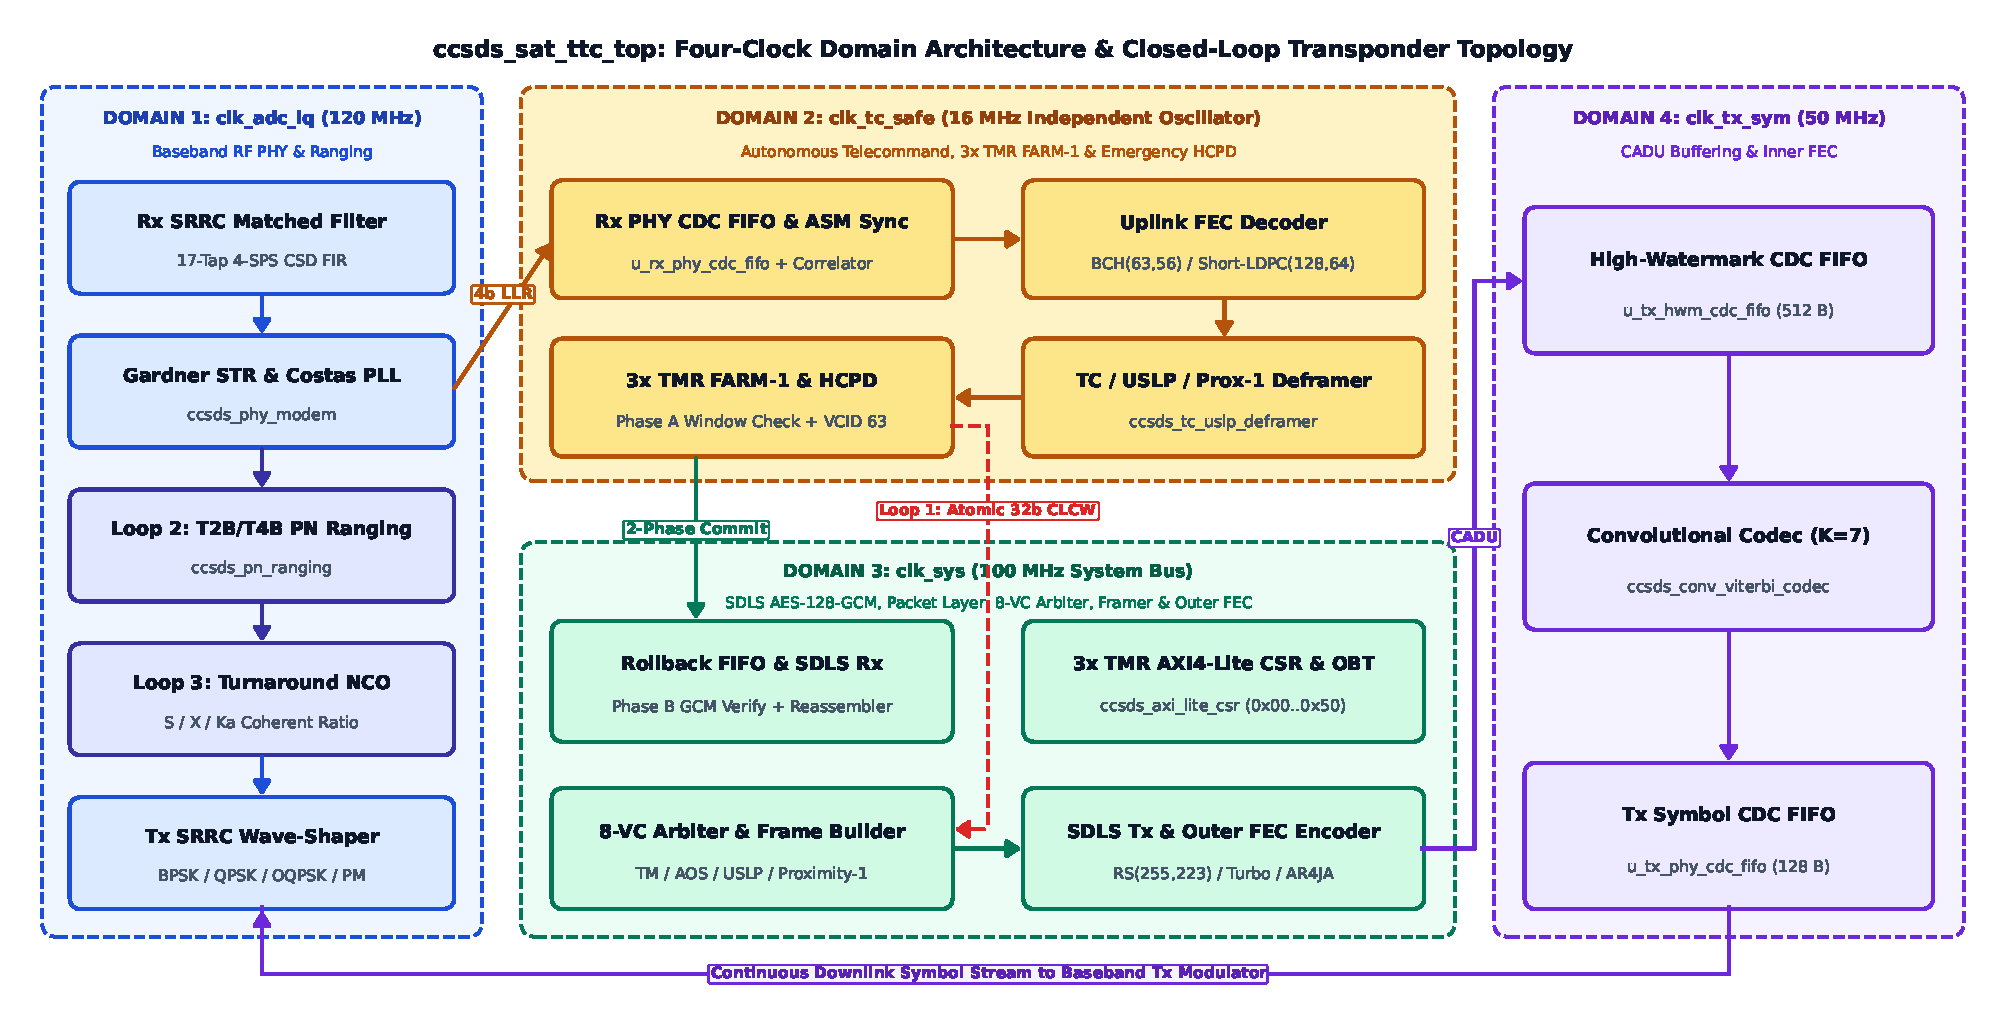
\includegraphics[width=0.95\textwidth]{docs/figures/fig1_top_level_architecture.pdf}
    \vspace{-4pt}
    \caption{\small Four-clock domain architecture and closed-loop transponder topology of \texttt{ccsds\_sat\_ttc\_top}.}
\end{figure}

\subsection{Seven-Stage Uplink \& Downlink Signal Flow}
\textbf{Figure~1.2} illustrates the end-to-end signal processing pipelines for an incoming uplink telecommand (\textbf{Stages U1--U7}) and an outgoing downlink telemetry frame (\textbf{Stages D1--D7}), together with the three closed-loop transponder paths connecting receiver to transmitter.

\begin{figure}[htbp]
    \centering
    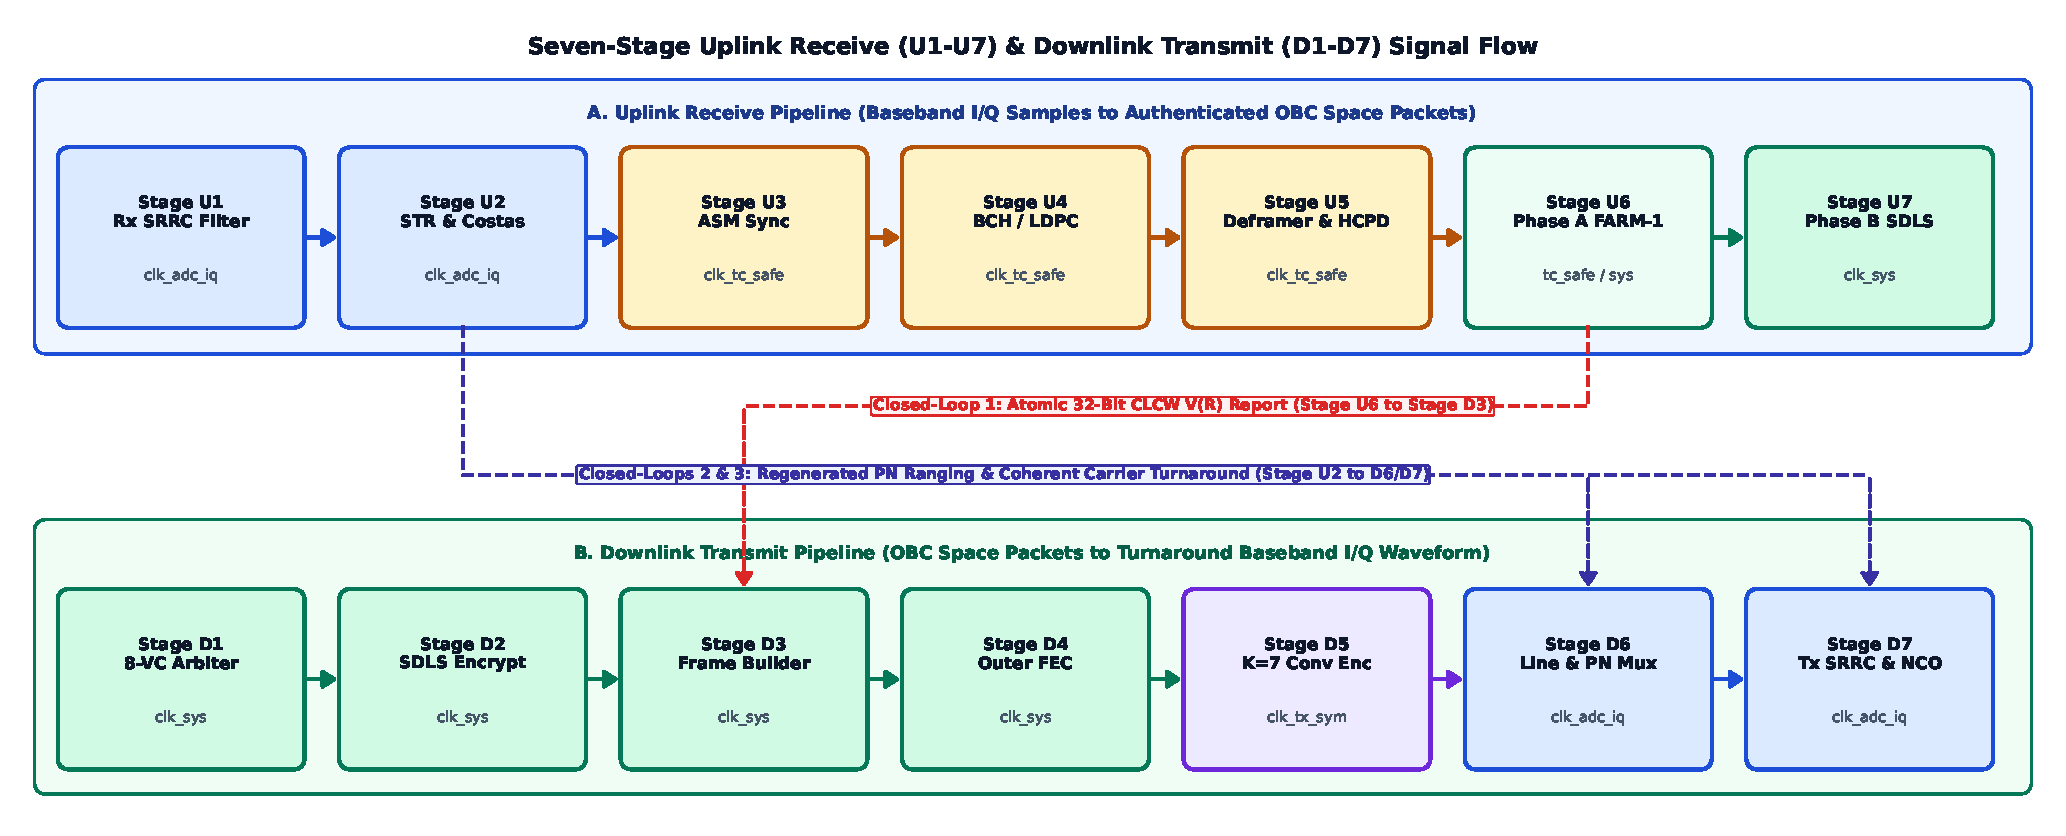
\includegraphics[width=0.98\textwidth]{docs/figures/fig_ul_dl_signal_flow.pdf}
    \vspace{-4pt}
    \caption{\small Seven-stage uplink receive pipeline (\texttt{U1--U7}), downlink transmit pipeline (\texttt{D1--D7}), and closed-loop transponder feedback paths.}
\end{figure}

\paragraph{A. Uplink Receive Pipeline (\texttt{Stages U1--U7}):}
\begin{enumerate}\setlength{\itemsep}{1.5pt}
    \item \textbf{\texttt{Stage U1} --- Baseband Filtering (\texttt{clk\_adc\_iq}, $120\,\text{MHz}$):} Complex NCO derotation and the 17-tap multiplier-free CSD 4-SPS SRRC matched filter ($\alpha=0.35$) in \texttt{ccsds\_phy\_modem.sv} strip out-of-band noise and close the Nyquist eye.
    \item \textbf{\texttt{Stage U2} --- Carrier, Timing \& Ranging Lock (\texttt{clk\_adc\_iq}):} An FLL-assisted PI Costas loop tracks carrier Doppler, a 3-stage Gardner TED slices 4-bit soft LLRs, and \texttt{ccsds\_pn\_ranging.sv} locks onto the \texttt{T2B}/\texttt{T4B} ranging sequence.
    \item \textbf{\texttt{Stage U3} --- CDC Crossing \& Frame Sync (\texttt{clk\_tc\_safe}, $16\,\text{MHz}$):} Soft LLRs cross via \texttt{u\_rx\_phy\_cdc\_fifo} into the independent telecommand clock domain, where \texttt{ccsds\_asm\_correlator.sv} resolves $0^\circ/180^\circ$ phase ambiguity.
    \item \textbf{\texttt{Stage U4} --- Uplink FEC \& Descrambling (\texttt{clk\_tc\_safe}):} Hardware straps (\texttt{ul\_fec\_override\_en}) select expurgated $\text{BCH}(63,56)$ SEC-DED or 4-phase $\text{Short-LDPC}(128,64)$ Soft-OMS decoding, followed by $h_{\text{TC}}(x)$ descrambling.
    \item \textbf{\texttt{Stage U5} --- Deframing \& Emergency \texttt{HCPD} (\texttt{clk\_tc\_safe}):} \texttt{ccsds\_tc\_uslp\_deframer.sv} strips \texttt{0x55} fill octets and checks CRC-16/32, while \texttt{VCID=63} frames branch directly to 3x TMR \texttt{ccsds\_hcpd\_ctrl.sv} for OBC hardware reset.
    \item \textbf{\texttt{Stage U6} --- Phase~A Window Check (\texttt{clk\_tc\_safe} $\to$ \texttt{clk\_sys}):} 3x TMR \texttt{ccsds\_farm1\_tmr.sv} verifies $N(S)$ against the sliding window while keeping $V(R)$ frozen and writes the candidate frame into \texttt{u\_rx\_commit\_cdc\_fifo}.
    \item \textbf{\texttt{Stage U7} --- Phase~B SDLS Verify \& Packet Release (\texttt{clk\_sys}, $100\,\text{MHz}$):} \texttt{ccsds\_sdls\_engine.sv} verifies the 128-bit \texttt{AES-128-GCM} tag; a valid tag commits $V(R)$ (\textbf{Closed-Loop \#1}) and releases packets on \texttt{m\_axis\_rx\_pkt\_*}, whereas a failed tag rolls back the FIFO pointer.
\end{enumerate}

\paragraph{B. Downlink Transmit Pipeline (\texttt{Stages D1--D7}):}
\begin{enumerate}\setlength{\itemsep}{1.5pt}
    \item \textbf{\texttt{Stage D1} --- Virtual Channel Arbitration (\texttt{clk\_sys}, $100\,\text{MHz}$):} \texttt{ccsds\_vc\_arbiter\_mux.sv} arbitrates across 8 VCs from \texttt{s\_axis\_tx\_pkt\_*} and computes the Cycle-0 \texttt{First\_Hdr\_Ptr} (\texttt{FHP}).
    \item \textbf{\texttt{Stage D2} --- Inline SDLS Encryption (\texttt{clk\_sys}):} \texttt{ccsds\_sdls\_engine.sv} encrypts the Transfer Frame Data Field using \texttt{AES-128-CTR/GCM} and appends the 128-bit \texttt{GHASH} authentication tag.
    \item \textbf{\texttt{Stage D3} --- Multi-Protocol Frame Assembly (\texttt{clk\_sys}):} \texttt{ccsds\_tm\_aos\_uslp\_framer.sv} attaches the Primary Header, 48-bit CUC \texttt{OBT}, live 32-bit \texttt{CLCW} (\textbf{Closed-Loop \#1}), and CRC-16/32 trailer.
    \item \textbf{\texttt{Stage D4} --- Outer FEC \& Randomization (\texttt{clk\_sys}):} \texttt{ccsds\_dl\_rs255\_223\_enc.sv} (or \texttt{ccsds\_dl\_turbo\_ldpc\_enc.sv}) and the $h_{\text{TM}}(x)$ scrambler form the Channel Access Data Unit (CADU).
    \item \textbf{\texttt{Stage D5} --- High-Watermark Buffering \& Inner FEC (\texttt{clk\_tx\_sym}, $50\,\text{MHz}$):} The 512-byte pre-fill FIFO \texttt{u\_tx\_hwm\_cdc\_fifo} feeds \texttt{ccsds\_conv\_viterbi\_codec.sv} ($r=1/2, K=7$) with zero underflow bubbles.
    \item \textbf{\texttt{Stage D6} --- Line Coding \& Ranging Overlay (\texttt{clk\_adc\_iq}, $120\,\text{MHz}$):} Symbols map to \texttt{NRZ-L/M} or \texttt{Bi-$\phi$-L} over \texttt{BPSK/QPSK/OQPSK/PCM-PM} with regenerated \texttt{T2B}/\texttt{T4B} ranging overlaid on the Q channel (\textbf{Closed-Loop \#2}).
    \item \textbf{\texttt{Stage D7} --- Polyphase SRRC Shaping \& Turnaround (\texttt{clk\_adc\_iq}):} The 17-tap polyphase SRRC filter and rational turnaround NCO (\textbf{Closed-Loop \#3}: S-Band $240/221$, X-Band $880/749$, or X$\to$Ka $3344/749, 3360/749, 3328/749$) drive \texttt{tx\_i/q\_dac\_out}.
\end{enumerate}

\subsection{RTL Module Inventory \& Standards Compliance}
\textbf{Table~1.1} organizes all 30 SystemVerilog files in \texttt{rtl/} and the 11 testbenches in \texttt{tb/} into five functional groups.

\begin{table}[htbp]
\centering
\scriptsize
\renewcommand{\arraystretch}{1.08}
\begin{tabularx}{\textwidth}{@{}L{1.82in}L{0.82in}C{0.68in}Y@{}}
\toprule
\textbf{SystemVerilog File Path} & \textbf{Clock Domain} & \textbf{\texttt{ROLE\_MODE}} & \textbf{Primary Hardware Function} \\
\midrule
\multicolumn{4}{@{}l}{\textbf{\color{navy}1. Shared Foundation, Math \& Clock-Domain Crossing Primitives (6 Files)}} \\
\texttt{rtl/ccsds\_pkg.sv} & All Domains & \texttt{0, 1, 2} & Packed protocol structs, $GF(2^8)$ dual-basis matrices, and FEC constants. \\
\texttt{rtl/ccsds\_crc\_universal.sv} & \texttt{clk\_sys / tc} & \texttt{0, 1, 2} & Single-cycle byte-wide CRC-16-CCITT (\texttt{0x1021}) and CRC-32 (\texttt{0x00A00805}). \\
\texttt{rtl/ccsds\_lfsr\_scrambler.sv} & \texttt{clk\_sys / tc} & \texttt{0, 1, 2} & 255-byte $h_{\text{TM}}(x)$ (\texttt{0xA9}) and $h_{\text{TC}}(x)$ (\texttt{0x5F}) additive randomizers. \\
\texttt{rtl/ccsds\_cdc\_fifo\_ecc.sv} & Dual-Clock & \texttt{0, 1, 2} & Gray-coded LUTRAM (\texttt{RAM64M}) CDC FIFO with Hsiao $(39,32)$ SECDED \& rollback. \\
\texttt{rtl/ccsds\_gf256\_math.sv} & \texttt{clk\_sys} & \texttt{0, 1, 2} & $GF(2^8)$ multiplier (\texttt{0x187}), dual-basis map, and AOS $GF(2^4)$ $\text{RS}(10,6)$ \texttt{FHEC}. \\
\texttt{rtl/ccsds\_axi\_lite\_csr.sv} & \texttt{clk\_sys} & \texttt{0, 1, 2} & 3x TMR AXI4-Lite CSR bank (\texttt{0x00..0x50}), 48-bit CUC \texttt{OBT}, and W1C counters. \\
\midrule
\multicolumn{4}{@{}l}{\textbf{\color{navy}2. Uplink Telecommand, Security, COP-1 ARQ \& Emergency Recovery Chain (9 Files)}} \\
\texttt{rtl/ccsds\_asm\_correlator.sv} & \texttt{clk\_tc\_safe} & \texttt{0, 1, 2} & Soft-LLR $0^\circ/180^\circ$ correlator for CLTU, TM/AOS, Proximity-1, and LDPC ASMs. \\
\texttt{rtl/ccsds\_bch6356\_dec.sv} & \texttt{clk\_tc\_safe} & \texttt{0, 2} & Spacecraft expurgated $\text{BCH}(63,56)$ SEC-DED decoder and CLTU tail detector. \\
\texttt{rtl/ccsds\_bch6356\_enc.sv} & \texttt{clk\_sys} & \texttt{1, 2} & Ground EGSE $\text{BCH}(63,56)$ CLTU encoder with \texttt{0x55} fill-octet padding. \\
\texttt{rtl/ccsds\_ul\_short\_ldpc\_dec.sv} & \texttt{clk\_tc\_safe} & \texttt{0, 2} & 4-phase 16-row/clk CCSDS 231.1-O-1 $(128,64)$ Soft-OMS iterative LDPC decoder. \\
\texttt{rtl/ccsds\_tc\_uslp\_deframer.sv} & \texttt{clk\_tc\_safe} & \texttt{0, 1, 2} & Uplink TC (\texttt{0x55} fill strip), Proximity-1, and USLP deframer + CRC checker. \\
\texttt{rtl/ccsds\_farm1\_tmr.sv} & \texttt{clk\_tc\_safe} & \texttt{0, 2} & 3x TMR COP-1 \texttt{FARM-1} responder with Two-Phase SDLS commit/rollback. \\
\texttt{rtl/ccsds\_hcpd\_ctrl.sv} & \texttt{clk\_tc\_safe} & \texttt{0, 2} & 3x TMR Emergency Command Decoder (\texttt{VCID=63}) driving OBC reset \& relays. \\
\texttt{rtl/ccsds\_sdls\_engine.sv} & \texttt{clk\_sys} & \texttt{0, 1, 2} & Inline \texttt{AES-128-CTR/GCM} ($GF(2^{128})$ 4b/clk \texttt{GHASH}) and 64-SA SECDED RAM. \\
\texttt{rtl/ccsds\_pkt\_reassembler.sv} & \texttt{clk\_sys} & \texttt{0, 1, 2} & Uplink Space Packet reassembler with automatic \texttt{APID 0x7FF} Idle stripping. \\
\midrule
\multicolumn{4}{@{}l}{\textbf{\color{navy}3. Downlink Telemetry, Framing, Ground EGSE \& Outer/Inner FEC Chain (9 Files)}} \\
\texttt{rtl/ccsds\_vc\_arbiter\_mux.sv} & \texttt{clk\_sys} & \texttt{0, 1, 2} & 8-VC priority/weighted arbiter and Cycle-0 closed-form \texttt{FHP} calculator. \\
\texttt{rtl/ccsds\_tm\_aos\_uslp\_framer.sv} & \texttt{clk\_sys} & \texttt{0, 1, 2} & Downlink TM (8B CUC \texttt{OBT}), AOS (\texttt{FHEC}), Proximity-1, and USLP frame builder. \\
\texttt{rtl/ccsds\_dl\_rs255\_223\_enc.sv} & \texttt{clk\_sys} & \texttt{0, 2} & Downlink dual-basis $\text{RS}(255,223)$ encoder ($I \in \{1..8\}$, virtual fill $Q$). \\
\texttt{rtl/ccsds\_dl\_rs255\_223\_dec.sv} & \texttt{clk\_sys} & \texttt{1, 2} & Ground EGSE $t=16$ Berlekamp-Massey, Chien, and Forney $\text{RS}(255,223)$ decoder. \\
\texttt{rtl/ccsds\_dl\_turbo\_ldpc\_enc.sv} & \texttt{clk\_sys} & \texttt{0, 2} & Downlink AR4JA quasi-cyclic LDPC and 16-state RSC Turbo ($r=1/2..1/6$) encoder. \\
\texttt{rtl/ccsds\_conv\_viterbi\_codec.sv} & \texttt{clk\_tx\_sym} & \texttt{0, 1, 2} & Rate-$1/2, K=7$ convolutional encoder (Tx) and 64-state soft Viterbi decoder (Rx). \\
\texttt{rtl/ccsds\_fop1\_engine.sv} & \texttt{clk\_sys} & \texttt{1, 2} & Ground EGSE COP-1 \texttt{FOP-1} initiator with Go-Back-$N$ retransmission queue. \\
\texttt{rtl/ccsds\_tc\_cltu\_framer.sv} & \texttt{clk\_sys} & \texttt{1, 2} & Ground EGSE TC Transfer Frame builder (40b Primary + 8b Segment + CRC-16). \\
\texttt{rtl/ccsds\_tm\_aos\_deframer.sv} & \texttt{clk\_sys} & \texttt{1, 2} & Ground EGSE TM/AOS deframer and CRC-gated 32-bit \texttt{CLCW} extractor. \\
\midrule
\multicolumn{4}{@{}l}{\textbf{\color{navy}4. Proximity-1 ARQ, Baseband RF Modem, PN Ranging \& Top-Level Wrapper (4 Files)}} \\
\texttt{rtl/ccsds\_prox1\_plcw\_ctrl.sv} & \texttt{clk\_sys} & \texttt{0, 1, 2} & Proximity-1 COP-P 32-bit \texttt{PLCW} sequence and retransmission controller. \\
\texttt{rtl/ccsds\_pn\_ranging.sv} & \texttt{clk\_adc\_iq} & \texttt{0, 1, 2} & Regenerative \texttt{T2B}/\texttt{T4B} 6-component PN ranging correlator ($L=1{,}009{,}470$). \\
\texttt{rtl/ccsds\_phy\_modem.sv} & \texttt{clk\_adc\_iq} & \texttt{0, 1, 2} & 17-tap CSD 4-SPS SRRC, Gardner STR, FLL/Costas PLL, and S/X/Ka turnaround. \\
\texttt{rtl/ccsds\_sat\_ttc\_top.sv} & All 4 Clocks & \texttt{0, 1, 2} & Parameterized top-level transceiver integrating all sub-cores and CDC bridges. \\
\midrule
\multicolumn{4}{@{}l}{\textbf{\color{navy}5. Orbital Channel Models \& Self-Checking Verification Suites (2 RTL + 11 TB Files)}} \\
\texttt{rtl/ccsds\_*\_channel\_model.sv} (2) & \texttt{clk\_adc\_iq} & Sim Model & Orbital S-curve Doppler, Rician fading, AWGN, multipath, and SSPA models. \\
\texttt{tb/tb\_stage2..12\_*.sv} (11 files) & Verification & Testbench & 11 self-checking testbenches + 34,560-trial full-chip RF matrix \& pass suite. \\
\bottomrule
\end{tabularx}
\caption{\footnotesize Grouped inventory of the 30 SystemVerilog modules in \texttt{rtl/} and 11 verification suites in \texttt{tb/}.}
\end{table}

Together, the synthesizable modules in \textbf{Table~1.1} implement 17 CCSDS Blue and Orange Book standards across packet formatting, data link framing, forward error correction, link security, timekeeping, and physical-layer modulation. \textbf{Table~1.2} maps each CCSDS specification to its corresponding RTL implementation.

\begin{table}[htbp]
\centering
\scriptsize
\renewcommand{\arraystretch}{1.10}
\begin{tabularx}{\textwidth}{@{}L{0.92in}L{1.58in}L{1.55in}Y@{}}
\toprule
\textbf{CCSDS Book} & \textbf{Standard Title} & \textbf{Primary RTL Module(s)} & \textbf{Hardware Implementation Summary} \\
\midrule
\multicolumn{4}{@{}l}{\textbf{\color{navy}1. Space Packet, Data Link Framing \& Closed-Loop ARQ Protocols}} \\
\href{https://ccsds.org/Pubs/133x0b2e1.pdf}{\textbf{133.0-B-2}} \cite{ccsds133} & Space Packet Protocol & \texttt{ccsds\_vc\_arbiter\_mux}, \texttt{pkt\_reasm} & 48-bit header check, Cycle-0 \texttt{FHP} segmentation, \texttt{APID 0x7FF} idle insert/strip. \\
\href{https://ccsds.org/Pubs/132x0b3.pdf}{\textbf{132.0-B-3}} \cite{ccsds132} & TM Space Data Link & \texttt{ccsds\_tm\_aos\_uslp\_framer/deframer} & 48-bit TM header, \texttt{MC/VC} counters, 8B CUC \texttt{OBT}, atomic 32-bit \texttt{CLCW}, CRC-16. \\
\href{https://ccsds.org/Pubs/232x0b4e1c1.pdf}{\textbf{232.0-B-4}} \cite{ccsds232} & TC Space Data Link & \texttt{ccsds\_tc\_uslp\_deframer}, \texttt{cltu\_framer} & 40-bit TC header, 8-bit Segment Header (\texttt{MAP\_ID}), \texttt{0x55} fill strip, Type-AD/BD/BC. \\
\href{https://ccsds.org/Pubs/232x1b2e2c1.pdf}{\textbf{232.1-B-2}} \cite{ccsds2321} & COP-1 (\texttt{FARM-1} / \texttt{FOP-1}) & \texttt{ccsds\_farm1\_tmr}, \texttt{ccsds\_fop1\_engine} & 3x TMR \texttt{FARM-1} (8 VCs, Two-Phase SDLS commit) and ground \texttt{FOP-1} Go-Back-$N$. \\
\href{https://ccsds.org/Pubs/732x0b4.pdf}{\textbf{732.0-B-4}} \cite{ccsds732} & AOS Space Data Link & \texttt{ccsds\_tm\_aos\_uslp\_framer}, \texttt{gf256} & 48-bit AOS header with 16-bit $GF(2^4)$ $\text{RS}(10,6)$ \texttt{FHEC} SEC-DED header protection. \\
\href{https://ccsds.org/Pubs/732x1b3.pdf}{\textbf{732.1-B-3}} \cite{ccsds7321} & Unified Space Link (USLP) & \texttt{ccsds\_tc\_uslp\_deframer}, \texttt{tm\_framer} & Truncated (32b) and Extended (56--112b) headers, 16b \texttt{SCID}, 24b \texttt{TFDFH}, CRC-16/32. \\
\href{https://ccsds.org/Pubs/211x0b6.pdf}{\textbf{211.0/1/2-B}} \cite{ccsds211} & Proximity-1 Space Link & \texttt{ccsds\_prox1\_plcw\_ctrl}, \texttt{crc\_univ} & Version-3 40-bit header, 24-bit ASM (\texttt{0xFAF320}), 32-bit \texttt{PLCW}, CRC-32 (\texttt{0x00A00805}). \\
\midrule
\multicolumn{4}{@{}l}{\textbf{\color{navy}2. Synchronization \& Channel Coding (Forward Error Correction)}} \\
\href{https://ccsds.org/Pubs/131x0b5.pdf}{\textbf{131.0-B-5}} \cite{ccsds131} & TM Sync \& Channel Coding & \texttt{rs255\_223}, \texttt{conv\_viterbi}, \texttt{turbo\_ldpc} & Dual-basis $\text{RS}(255,223)$ ($I \in \{1..8\}, Q$), $K=7$ Conv/Viterbi, 16-state Turbo, $h_{\text{TM}}$. \\
\href{https://ccsds.org/Pubs/231x0b4e1.pdf}{\textbf{231.0-B-4}} \cite{ccsds231} & TC Sync \& Channel Coding & \texttt{ccsds\_bch6356\_dec/enc}, \texttt{hcpd\_ctrl} & CLTU (\texttt{0xEB90}), expurgated $\text{BCH}(63,56)$ SEC-DED, Tail (\texttt{0xC5..79}), $h_{\text{TC}}$, 3x TMR \texttt{HCPD}. \\
\href{https://ccsds.org/Pubs/231x1o1s.pdf}{\textbf{231.1-O-1}} \cite{ccsds2311} & Uplink Short-Block LDPC & \texttt{ccsds\_ul\_short\_ldpc\_dec.sv} & Quasi-cyclic $(128,64)$ LDPC with 4-phase 16-row/clk Soft-OMS iterative decoder. \\
\midrule
\multicolumn{4}{@{}l}{\textbf{\color{navy}3. Link Security, Timekeeping, RF Modulation \& Ranging}} \\
\href{https://ccsds.org/Pubs/301x0b4e1.pdf}{\textbf{301.0-B-4}} \cite{ccsds301} & CUC Time Code Formats & \texttt{ccsds\_axi\_lite\_csr.sv} & 48-bit CUC \texttt{OBT} (32b Coarse + 16b Fine, P-Field \texttt{0x2E}) locked to \texttt{pps\_1hz\_in}. \\
\href{https://ccsds.org/Pubs/355x0b2.pdf}{\textbf{355.0/1-B}} \cite{ccsds355} & Space Data Link Security & \texttt{ccsds\_sdls\_engine.sv} & NIST \texttt{AES-128-CTR} \& \texttt{AES-128-GCM} ($GF(2^{128})$ 128b \texttt{GHASH} tag) + 64-SA RAM. \\
\href{https://ccsds.org/Pubs/401x0b32.pdf}{\textbf{401.0-B-32}} \cite{ccsds401} & RF \& Modulation Systems & \texttt{ccsds\_phy\_modem.sv} & \texttt{BPSK/QPSK/OQPSK/PCM-PM}, 17-tap 4-SPS CSD SRRC, Gardner STR, S/X/Ka ratios. \\
\href{https://ccsds.org/Pubs/414x1b3e1.pdf}{\textbf{414.1-B-3}} \cite{ccsds414} & Pseudo-Noise Ranging & \texttt{ccsds\_pn\_ranging.sv} & 6-component weighted-voting \texttt{T2B}/\texttt{T4B} correlator ($L=1{,}009{,}470$) \& Q-channel overlay. \\
\bottomrule
\end{tabularx}
\caption{\footnotesize Grouped CCSDS Blue and Orange Book compliance matrix for \texttt{ccsds\_sat\_ttc\_top (v2.40.3)}.}
\end{table}

% =============================================================================
% CHAPTER 2: PRODUCT SPECIFICATION, CLOCKING, RESETS & RESOURCE UTILIZATION
% =============================================================================
\vspace{6pt}
\section{Product Specification, Clocking \& Resource Footprint}

Having traced the functional signal flow across the transceiver in Chapter~1, we now specify the physical FPGA integration parameters required to instantiate \texttt{ccsds\_sat\_ttc\_top}. This chapter details each compile-time synthesis generic and its legal values, explains why the architecture is partitioned across four isolated clock domains, defines the reset and 1-PPS timing requirements, and reports measured Logic LUT, Distributed LUTRAM (\texttt{RAM64M}), and Flip-Flop resource utilization and static timing closure.

\subsection{Compile-Time Synthesis Generics}
To allow avionics designers to trade off optional protocol features against FPGA LUT footprint without editing RTL source files, \texttt{ccsds\_sat\_ttc\_top} exposes four compile-time SystemVerilog parameters. In \textbf{Table~2.1}, every legal parameter value is given its own dedicated row to clearly show which sub-modules are elaborated or pruned and how FPGA logic resources are affected.

\begin{table}[htbp]
\centering
\scriptsize
\renewcommand{\arraystretch}{1.20}
\begin{tabularx}{\textwidth}{@{}L{1.15in}C{0.55in}C{0.52in}L{1.65in}Y@{}}
\toprule
\textbf{Parameter Name} & \textbf{Value} & \textbf{Default?} & \textbf{Elaborated / Pruned RTL Scope} & \textbf{Hardware Synthesis \& Resource Impact} \\
\midrule
\texttt{ROLE\_MODE} & \texttt{0} & \textbf{Yes} & \textbf{Spacecraft Flight Persona} (23 modules elaborated; 5 ground modules pruned) & Synthesizes spacecraft Rx decoders (\texttt{BCH}, \texttt{LDPC}, \texttt{FARM-1}, \texttt{HCPD}) and Tx encoders (\texttt{RS}, \texttt{Turbo}). Prunes ground \texttt{FOP-1}, \texttt{CLTU} enc, and $t=16$ \texttt{RS} dec. \\
\texttt{ROLE\_MODE} & \texttt{1} & No & \textbf{Hardware Ground EGSE Persona} (22 modules elaborated; 6 flight modules pruned) & Synthesizes ground Tx (\texttt{FOP-1} Go-Back-$N$, \texttt{TC/CLTU} enc) and ground Rx ($t=16$ Berlekamp-Massey \texttt{RS} dec, \texttt{TM/AOS} deframer with \texttt{CLCW} extractor). \\
\texttt{ROLE\_MODE} & \texttt{2} & No & \textbf{Universal Crosslink \& BIST Persona} (All 28 synthesizable modules elaborated) & Instantiates both spacecraft flight and ground EGSE endpoints simultaneously for Proximity-1/USLP crosslinks and autonomous on-orbit loopback BIST. \\
\midrule
\texttt{ENABLE\_SDLS} & \texttt{1'b1} & \textbf{Yes} & Elaborates \texttt{ccsds\_sdls\_engine.sv} (\texttt{g\_sdls\_engine}) & Includes full NIST FIPS-197 \texttt{AES-128-CTR}, NIST SP 800-38D \texttt{AES-128-GCM} ($GF(2^{128})$ \texttt{GHASH}), and 64-entry Hsiao $(39,32)$ SECDED SA RAM. \\
\texttt{ENABLE\_SDLS} & \texttt{1'b0} & No & Elaborates zero-latency wire bypass (\texttt{g\_no\_sdls\_engine}) & Physically elides the cryptographic engine and 64-SA RAM, hardwiring \texttt{sdls\_auth\_ok = 1'b1}. \textbf{Saves 7,919 Slice LUTs and 5,571 Slice FFs.} \\
\midrule
\texttt{ENABLE\_UL\_LDPC} & \texttt{1'b1} & \textbf{Yes} & Elaborates \texttt{ccsds\_ul\_short\_ldpc\_dec.sv} (\texttt{g\_ul\_ldpc\_dec}) & Includes the 4-phase 16-row/clk CCSDS 231.1-O-1 $(128,64)$ Soft-OMS iterative uplink LDPC decoder alongside $\text{BCH}(63,56)$. \\
\texttt{ENABLE\_UL\_LDPC} & \texttt{1'b0} & No & Prunes \texttt{ccsds\_ul\_short\_ldpc\_dec.sv} (\texttt{g\_no\_ul\_ldpc\_dec}) & Hardwires \texttt{ldpc\_dec\_tvalid = 1'b0} for classic $\text{BCH}(63,56)$-only missions. \textbf{Saves 12,610 Slice LUTs and 1,132 Slice FFs.} \\
\midrule
\texttt{IQ\_BUS\_WIDTH} & \texttt{16} & \textbf{Yes} & Elaborates 16-bit MSB-padded container mode & Exposes 16-bit signed \texttt{rx\_i/q\_adc\_in[15:0]} (slicing \texttt{[11:0]} internally) and \texttt{tx\_i/q\_dac\_out[15:0]} (padding \texttt{\{phy\_tx\_12b, 4'b0000\}} into \texttt{[15:4]}). \\
\texttt{IQ\_BUS\_WIDTH} & \texttt{12} & No & Elaborates direct 12-bit Q1.11 mode & Exposes direct 12-bit signed \texttt{rx\_i/q\_adc\_in[11:0]} and \texttt{tx\_i/q\_dac\_out[11:0]} ports matching the internal \texttt{ccsds\_phy\_modem} bit width 1:1. \\
\bottomrule
\end{tabularx}
\caption{\footnotesize Complete Compile-Time Synthesis Generics and Per-Value Elaboration Behavior in \texttt{rtl/ccsds\_sat\_ttc\_top.sv}.}
\end{table}

\subsection{Four-Clock Architecture \& CDC Isolation}
In a flight-qualified spacecraft transponder, clocking the emergency command receiver from the same Phase-Locked Loop (PLL) as the On-Board Computer bus creates a single-point failure: if an OBC clock synthesizer unlocks or stalls, the satellite becomes uncommandable. To eliminate this hazard and match each pipeline stage to its natural physical rate, \texttt{ccsds\_sat\_ttc\_top} partitions its logic across four asynchronous clock domains (\textbf{Table~2.2}) joined by Gray-coded Hsiao $(39,32)$ SECDED Distributed-LUTRAM FIFOs and 4-phase Request/Acknowledge handshakes.

\begin{table}[htbp]
\centering
\scriptsize
\renewcommand{\arraystretch}{1.18}
\begin{tabularx}{\textwidth}{@{}L{0.82in}C{0.72in}C{0.84in}C{0.84in}Y@{}}
\toprule
\textbf{Clock Port} & \textbf{Nominal} & \textbf{Zynq-7010 ($-1L$)} & \textbf{Kintex US} & \textbf{Domain Scope, Clock Source \& CDC Isolation Strategy} \\
\midrule
\texttt{clk\_adc\_iq} & $120.0\,\text{MHz}$ & $135.41\,\text{MHz}$ & $271.74\,\text{MHz}$ & Driven by the external baseband ADC/DAC or SDR transceiver sample clock. Clocks \texttt{ccsds\_phy\_modem.sv} (4-SPS SRRC, Gardner STR, Costas loop, turnaround NCO) and \texttt{ccsds\_pn\_ranging.sv}. Crosses to \texttt{clk\_tc\_safe} via \texttt{u\_rx\_phy\_cdc\_fifo}. \\
\texttt{clk\_tc\_safe} & $16.0\,\text{MHz}$ & $110.22\,\text{MHz}$ & $203.38\,\text{MHz}$ & Driven by an independent crystal oscillator dedicated to the Uplink Telecommand chain (\texttt{ccsds\_asm\_correlator}, \texttt{ccsds\_bch6356\_dec}, \texttt{ccsds\_ul\_short\_ldpc\_dec}, \texttt{ccsds\_tc\_uslp\_deframer}, 3x TMR \texttt{FARM-1}, and 3x TMR \texttt{HCPD}). Operates even if \texttt{clk\_sys} halts. \\
\texttt{clk\_sys} & $100.0\,\text{MHz}$ & $116.40\,\text{MHz}$ & $217.34\,\text{MHz}$ & Main OBC \texttt{AXI4-Lite} CSR and \texttt{AXI4-Stream} Space Packet clock. Clocks \texttt{ccsds\_axi\_lite\_csr}, \texttt{ccsds\_sdls\_engine}, \texttt{ccsds\_pkt\_reassembler}, \texttt{ccsds\_vc\_arbiter\_mux}, \texttt{ccsds\_tm\_aos\_uslp\_framer}, and \texttt{ccsds\_dl\_rs255\_223\_enc}. \\
\texttt{clk\_tx\_sym} & $50.0\,\text{MHz}$ & $169.46\,\text{MHz}$ & $232.50\,\text{MHz}$ & Downlink symbol/CADU clock. Driven from \texttt{clk\_sys} via the 512-byte High-Watermark Pre-Fill asynchronous SECDED FIFO (\texttt{u\_tx\_hwm\_cdc\_fifo}) so the convolutional encoder and modulator never experience an underflow bubble. \\
\bottomrule
\end{tabularx}
\caption{\footnotesize Clock Domains, Nominal Targets, and Measured Two-Pass True $F_{\max}$ Across Slowest-Grade Zynq-7010 (\texttt{-1L}) and Kintex UltraScale (\texttt{XQRKU060}).}
\end{table}

\subsection{Reset Sequencing \& 1-PPS Time Synchronization}
Proper initialization across all four asynchronous clock domains is handled internally by dedicated reset synchronizers, while spacecraft timekeeping is maintained by a hardware 1-PPS synchronization circuit:
\begin{itemize}\setlength{\itemsep}{2.5pt}
    \item \textbf{Per-Domain 2-FF Reset Bridges (\texttt{rst\_n}):} The single active-low master reset pin \texttt{rst\_n} feeds four independent 2-flip-flop asynchronous-assert, synchronous-deassert reset synchronizer bridges (\texttt{rst\_sys\_n}, \texttt{rst\_tc\_n}, \texttt{rst\_tx\_n}, \texttt{rst\_adc\_n} marked with \texttt{(* ASYNC\_REG = "TRUE" *)}). During power-up or watchdog reset, hold \texttt{rst\_n == 1'b0} for at least \textbf{8 cycles of the slowest clock (\texttt{clk\_tc\_safe}, $\ge 500\,\text{ns}$ at $16\,\text{MHz}$)} to guarantee clean, recovery/removal-safe deassertion across all four domains.
    \item \textbf{External 1-PPS Synchronization with Autonomous Internal Fallback (\texttt{pps\_1hz\_in}):} The 48-bit CCSDS 301.0-B-4 Unsegmented Time Code (\texttt{OBT}) counter in \texttt{ccsds\_axi\_lite\_csr.sv} increments its 32-bit coarse seconds register (\texttt{0x10}) on each rising edge of \texttt{pps\_1hz\_in} (synchronized into \texttt{clk\_sys} via a 2-FF \texttt{ASYNC\_REG} bridge). If the external GNSS or atomic clock 1-PPS signal is absent or interrupted for $>1.05\,\text{s}$ (\texttt{105,000,000} cycles of \texttt{clk\_sys}), an internal $100\,\text{MHz}$ hardware divider automatically takes over $1\,\text{Hz}$ coarse-second ticking while smoothly incrementing the 16-bit fine sub-seconds register (\texttt{0x14}, $15.26\,\mu\text{s}$ resolution).
\end{itemize}

\subsection{Distributed LUTRAM Footprint \& Timing Closure}
To eliminate Block RAM and DSP hard-macro Single-Event Functional Interrupts (SEFIs) while keeping flip-flop count under 14,000 FFs, \texttt{ccsds\_sat\_ttc\_top} applies three synthesis-level design techniques (\textbf{Tables~2.3--2.4}):
\begin{itemize}\setlength{\itemsep}{2pt}
    \item \textbf{Synchronous Distributed LUTRAM Inference (\texttt{1,200 LUTRAMs}):} In \texttt{rtl/ccsds\_cdc\_fifo\_ecc.sv}, the 39-bit FIFO arrays (\texttt{mem\_ecc\_reg}) use a synchronous write process (\texttt{always\_ff @(posedge clk\_wr)} with no asynchronous reset), mapping all CDC and 8-VC staging buffers into \texttt{RAM64M}/\texttt{RAM32M} SLICEM primitives rather than discrete flip-flops.
    \item \textbf{Continuous Combinational Hsiao $(39,32)$ SECDED Scrubbing:} Every 32-bit word read from Distributed LUTRAM is verified and corrected on the fly by a 7-bit odd-weight Hsiao SEC-DED syndrome decoder.
    \item \textbf{Multiplier-Free CSD Shift-Add DSP (\texttt{0 DSP48}):} All 17-tap SRRC filters and $GF(2^{128})$ \texttt{GHASH} multipliers use binary Canonical Signed-Digit (CSD) adder trees and 4-bit/clock LUT6 XOR steps.
\end{itemize}

\begin{table}[htbp]
\centering
\scriptsize
\renewcommand{\arraystretch}{1.18}
\begin{tabularx}{\textwidth}{@{}L{1.52in}C{0.78in}C{0.58in}C{0.58in}C{0.62in}C{0.68in}Y@{}}
\toprule
\textbf{Synthesis Profile (\texttt{ROLE=0})} & \textbf{Total LUTs (Logic + LUTRAM)} & \textbf{Slice FFs} & \textbf{BRAM / DSP} & \textbf{Zynq-7020 (\texttt{53.2k} LUT6)} & \textbf{Kintex US (\texttt{XQRKU060})} & \textbf{Lattice MachXO5-NX (\texttt{LFMXO5-100T}, \texttt{80k} LUT4)} \\
\midrule
\textbf{Full Flight (\texttt{SDLS=1, LDPC=1})} & \textbf{28,861} ($27.6\text{k} + 1.2\text{k}$) & \textbf{13,864} & \textbf{0 / 0} & \textbf{54.25\%} & \textbf{8.70\%} & \textbf{$\sim$46.8\%} ($\sim 37.5\text{k}$ LUT4) \\
\textbf{BCH + GCM (\texttt{SDLS=1, LDPC=0})} & \textbf{16,251} ($15.0\text{k} + 1.2\text{k}$) & \textbf{12,732} & \textbf{0 / 0} & \textbf{30.55\%} & \textbf{4.90\%} & \textbf{$\sim$26.4\%} ($\sim 21.1\text{k}$ LUT4) \\
\textbf{Compact (\texttt{SDLS=0, LDPC=0})} & \textbf{8,332} ($7.1\text{k} + 1.2\text{k}$) & \textbf{7,161} & \textbf{0 / 0} & \textbf{15.66\%} & \textbf{2.51\%} & \textbf{$\sim$13.5\%} ($\sim 10.8\text{k}$ LUT4) \\
\bottomrule
\end{tabularx}
\caption{\footnotesize Measured Synthesis Resource Utilization (Logic LUTs + 1,200 Distributed \texttt{RAM64M} LUTRAMs + Slice Flip-Flops, \texttt{0 BRAM / 0 DSP}).}
\end{table}

\begin{table}[htbp]
\centering
\scriptsize
\renewcommand{\arraystretch}{1.18}
\begin{tabularx}{\textwidth}{@{}L{0.72in}C{0.82in}C{0.72in}C{0.76in}C{0.35in}Y@{}}
\toprule
\textbf{Clock Domain} & \textbf{Nominal Target} & \textbf{Zynq-7010 ($-1L$) True $F_{\max}$} & \textbf{Kintex US True $F_{\max}$} & \textbf{Logic Levels} & \textbf{Limiting Physical Critical Path (\texttt{Vivado 2022.2 STA})} \\
\midrule
\texttt{clk\_sys} & $100.0\,\text{MHz}$ ($10.0\,\text{ns}$) & $\mathbf{116.40\,\text{MHz}}$ ($8.59\,\text{ns}$) & $\mathbf{217.34\,\text{MHz}}$ ($4.60\,\text{ns}$) & \textbf{7} & \texttt{\detokenize{u_rx_commit_cdc_fifo/rd_ptr_q[0]}} $\rightarrow$ \texttt{\detokenize{u_csr/cnt_uncorr_err_q[0]}} \\
\texttt{clk\_adc\_iq} & $120.0\,\text{MHz}$ ($8.33\,\text{ns}$) & $\mathbf{135.41\,\text{MHz}}$ ($7.39\,\text{ns}$) & $\mathbf{271.74\,\text{MHz}}$ ($3.68\,\text{ns}$) & \textbf{9} & \texttt{\detokenize{u_phy_modem/rx_phase_q16[10]}} $\rightarrow$ \texttt{\detokenize{u_phy_modem/i_derot_q[13]}} \\
\texttt{clk\_tx\_sym} & $50.0\,\text{MHz}$ ($20.0\,\text{ns}$) & $\mathbf{169.46\,\text{MHz}}$ ($5.90\,\text{ns}$) & $\mathbf{232.50\,\text{MHz}}$ ($4.30\,\text{ns}$) & \textbf{9} & \texttt{\detokenize{u_tx_hwm_cdc_fifo/wr_sync2[1]}} $\rightarrow$ \texttt{\detokenize{u_tx_hwm_cdc_fifo/rd_gray[6]}} \\
\texttt{clk\_tc\_safe} & $16.0\,\text{MHz}$ ($62.5\,\text{ns}$) & $\mathbf{110.22\,\text{MHz}}$ ($9.07\,\text{ns}$) & $\mathbf{203.38\,\text{MHz}}$ ($4.92\,\text{ns}$) & \textbf{11} & \texttt{\detokenize{u_ul_deframer/cur_tc_hdr[vcid]}} $\rightarrow$ \texttt{\detokenize{u_farm1/clcw_scheduled_out}} \\
\bottomrule
\end{tabularx}
\caption{\footnotesize Two-Pass Static Timing Analysis (STA) Across Slowest-Grade Zynq-7010 (\texttt{-1L}) and Radiation-Tolerant Kintex UltraScale (\texttt{XQRKU060}).}
\end{table}

% =============================================================================
% CHAPTER 3: HARDWARE SIGNAL INTERFACES & AXI4-STREAM SIDEBAND BUS
% =============================================================================
\vspace{6pt}
\section{Signal Dictionary, Sideband Bus \& I/Q Alignment}

To integrate \texttt{ccsds\_sat\_ttc\_top} into a top-level FPGA design, the hardware engineer connects seven logical signal groups: clocks and resets, the AXI4-Lite control bus, hardware mission straps, the baseband I/Q ADC/DAC interface, the AXI4-Stream OBC packet ingress and egress buses, the optional downlink CADU tap, and the emergency \texttt{HCPD} and fault outputs. This chapter provides the complete top-level port and signal dictionary (59 ports), defines the 64-bit \texttt{ccsds\_tuser\_t} sideband bus bit-by-bit, explains how to adapt the baseband I/Q port to any converter bit width or alignment convention, and explains why uplink FEC is controlled by hardware straps rather than software registers.

\subsection{Top-Level Port Reference (59 Ports)}
\textbf{Table~3.1} documents all 59 top-level ports of \texttt{ccsds\_sat\_ttc\_top} (\texttt{rtl/ccsds\_sat\_ttc\_top.sv}), grouped by functional interface.

{\scriptsize
\renewcommand{\arraystretch}{1.12}
\begin{longtable}{@{}L{1.82in}C{0.40in}C{0.46in}C{0.60in}L{2.85in}@{}}
\caption{\footnotesize Complete Pinout Reference for \texttt{ccsds\_sat\_ttc\_top} (\texttt{v2.40.3}).}\\
\toprule
\textbf{Port Name} & \textbf{Dir} & \textbf{Width} & \textbf{Clock} & \textbf{Functional Description \& Integration Notes} \\
\midrule
\endfirsthead
\toprule
\textbf{Port Name} & \textbf{Dir} & \textbf{Width} & \textbf{Clock} & \textbf{Functional Description \& Integration Notes} \\
\midrule
\endhead
\bottomrule
\endfoot
\multicolumn{5}{@{}l}{\textbf{\color{navy}1. Clocks, Reset \& 1-PPS Time Synchronization Interface}} \\
\texttt{clk\_sys} & In & 1 & \texttt{clk\_sys} & System packet, framing, CSR, SDLS \& outer FEC clock ($100\,\text{MHz}$ nominal). \\
\texttt{clk\_tc\_safe} & In & 1 & \texttt{clk\_tc\_safe} & Independent radiation-safe telecommand \& \texttt{HCPD} clock ($16\,\text{MHz}$ nominal). \\
\texttt{clk\_tx\_sym} & In & 1 & \texttt{clk\_tx\_sym} & Downlink symbol \& inner coding clock ($50\,\text{MHz}$ nominal). \\
\texttt{clk\_adc\_iq} & In & 1 & \texttt{clk\_adc\_iq} & Baseband RF ADC/DAC \& PN ranging sample clock ($120\,\text{MHz}$ nominal). \\
\texttt{rst\_n} & In & 1 & Async & Active-low master reset; hold low $\ge 8$ \texttt{clk\_tc\_safe} cycles ($\ge 500\,\text{ns}$). \\
\texttt{pps\_1hz\_in} & In & 1 & Async & External $1\,\text{Hz}$ (1-PPS) pulse for 48-bit CUC \texttt{OBT}; auto-fallback if idle $>1.05\,\text{s}$. \\
\midrule
\multicolumn{5}{@{}l}{\textbf{\color{navy}2. AXI4-Lite Control \& Status Register (CSR) Slave Interface (\texttt{0x00..0x50})}} \\
\texttt{s\_axi\_awvalid / s\_axi\_awready} & In/Out & 1, 1 & \texttt{clk\_sys} & AXI4-Lite write address valid/ready handshake. \\
\texttt{s\_axi\_awaddr} & In & 8 & \texttt{clk\_sys} & AXI4-Lite byte write address (\texttt{0x00..0x50}, 32-bit word aligned). \\
\texttt{s\_axi\_wvalid / s\_axi\_wready} & In/Out & 1, 1 & \texttt{clk\_sys} & AXI4-Lite write data valid/ready handshake. \\
\texttt{s\_axi\_wdata / s\_axi\_wstrb} & In & 32, 4 & \texttt{clk\_sys} & 32-bit write data bus and 4-bit byte-lane write strobe (\texttt{4'hF}). \\
\texttt{s\_axi\_bvalid / s\_axi\_bready} & Out/In & 1, 1 & \texttt{clk\_sys} & AXI4-Lite write response valid/ready handshake. \\
\texttt{s\_axi\_bresp} & Out & 2 & \texttt{clk\_sys} & Write response status (\texttt{2'b00 = OKAY}). \\
\texttt{s\_axi\_arvalid / s\_axi\_arready} & In/Out & 1, 1 & \texttt{clk\_sys} & AXI4-Lite read address valid/ready handshake. \\
\texttt{s\_axi\_araddr} & In & 8 & \texttt{clk\_sys} & AXI4-Lite byte read address (\texttt{0x00..0x50}). \\
\texttt{s\_axi\_rvalid / s\_axi\_rready} & Out/In & 1, 1 & \texttt{clk\_sys} & AXI4-Lite read data valid/ready handshake. \\
\texttt{s\_axi\_rdata / s\_axi\_rresp} & Out & 32, 2 & \texttt{clk\_sys} & 32-bit read data bus and read response status (\texttt{2'b00 = OKAY}). \\
\midrule
\multicolumn{5}{@{}l}{\textbf{\color{navy}3. Hardware Mission Straps \& Physical Mode Overrides}} \\
\texttt{link\_proto\_override\_en} & In & 2 & \texttt{clk\_sys} & \texttt{2'b00}: Use CSR \texttt{0x04[14:12]}; non-zero overrides protocol mode in hardware. \\
\texttt{ul\_fec\_override\_en} & In & 2 & \texttt{clk\_tc\_safe} & Uplink FEC strap: \texttt{2'd0}=Uncoded, \texttt{2'd1}=$\text{BCH}(63,56)$, \texttt{2'd2}=$\text{LDPC}(128,64)$. \\
\texttt{sdls\_en\_cfg / bc\_require\_sdls\_cfg} & In & 1, 1 & \texttt{clk\_sys} & Mission security straps OR-ed with CSR \texttt{0x04[26]} and \texttt{0x04[27]}. \\
\texttt{pn\_ranging\_en\_cfg / pn\_t4b\_mode\_cfg} & In & 1, 1 & \texttt{clk\_adc\_iq} & Enable regenerative PN ranging (\texttt{1}) and select \texttt{T4B} (\texttt{1}) vs.\ \texttt{T2B} (\texttt{0}) voting. \\
\texttt{turnaround\_xband\_cfg} & In & 1 & \texttt{clk\_adc\_iq} & Selects S-Band $240/221$ (\texttt{0}) or X-Band $880/749$ (\texttt{1}) when X$\to$Ka CSR is \texttt{0}. \\
\texttt{mod\_mode\_cfg / line\_code\_cfg} & In & 2, 2 & \texttt{clk\_adc\_iq} & Modulation (\texttt{0=BPSK, 1=QPSK, 2=OQPSK, 3=PCM/PM}) \& Line Code (\texttt{0..2}). \\
\midrule
\multicolumn{5}{@{}l}{\textbf{\color{navy}4. Uplink Baseband RF I/Q ADC \& Direct Symbol Bypass Inputs}} \\
\texttt{rx\_i\_adc\_in / rx\_q\_adc\_in} & In & $W, W$ & \texttt{clk\_adc\_iq} & Signed two's-complement I/Q ADC bus ($W = \texttt{IQ\_BUS\_WIDTH}$, default 16). \\
\texttt{rx\_iq\_valid\_in} & In & 1 & \texttt{clk\_adc\_iq} & Sample valid qualifier (supports decimated symbol rates $\text{div}=1,2,4,8$). \\
\texttt{s\_axis\_ul\_sym\_tvalid / tready} & In/Out & 1, 1 & \texttt{clk\_tc\_safe} & Direct baseband symbol/byte bypass ingress handshake (tie \texttt{tvalid=0} for RF). \\
\texttt{s\_axis\_ul\_sym\_tdata / tlast} & In & 8, 1 & \texttt{clk\_tc\_safe} & Signed 4-bit LLR (\texttt{tdata[3:0]}) or uncoded frame byte + end-of-frame strobe. \\
\midrule
\multicolumn{5}{@{}l}{\textbf{\color{navy}5. OBC AXI4-Stream Space Packet Egress (\texttt{m\_axis\_rx\_pkt}) \& Ingress (\texttt{s\_axis\_tx\_pkt})}} \\
\texttt{m\_axis\_rx\_pkt\_tvalid / tready} & Out/In & 1, 1 & \texttt{clk\_sys} & Reassembled \& authenticated Uplink Space Packet egress handshake to OBC. \\
\texttt{m\_axis\_rx\_pkt\_tdata / tlast} & Out & 8, 1 & \texttt{clk\_sys} & Uplink Space Packet byte stream; \texttt{tlast=1} marks final octet of packet. \\
\texttt{m\_axis\_rx\_pkt\_tuser} & Out & 64 & \texttt{clk\_sys} & Packed \texttt{ccsds\_tuser\_t} metadata (\texttt{vcid}, \texttt{map\_id}, \texttt{spi\_idx}, error flags; \textbf{Table~3.2}). \\
\texttt{s\_axis\_tx\_pkt\_tvalid / tready} & In/Out & 1, 1 & \texttt{clk\_sys} & Downlink Telemetry Space Packet ingress handshake from OBC. \\
\texttt{s\_axis\_tx\_pkt\_tdata / tlast} & In & 8, 1 & \texttt{clk\_sys} & Downlink Space Packet byte stream; \texttt{tlast=1} required on final packet octet. \\
\texttt{s\_axis\_tx\_pkt\_tuser} & In & 64 & \texttt{clk\_sys} & Ingress metadata (\texttt{tuser[47:42] = vcid} selects target Virtual Channel \texttt{0..7}). \\
\midrule
\multicolumn{5}{@{}l}{\textbf{\color{navy}6. Downlink CADU Byte Stream \& Baseband RF I/Q DAC Outputs}} \\
\texttt{m\_axis\_dl\_cad\_tvalid / tready} & Out/In & 1, 1 & \texttt{clk\_tx\_sym} & Scrambled \& outer-FEC encoded Downlink CADU byte stream (for external PHY). \\
\texttt{m\_axis\_dl\_cad\_tdata / tlast} & Out & 8, 1 & \texttt{clk\_tx\_sym} & Downlink CADU octet and end-of-CADU boundary strobe. \\
\texttt{tx\_i\_dac\_out / tx\_q\_dac\_out} & Out & $W, W$ & \texttt{clk\_adc\_iq} & Signed two's-complement I/Q DAC outputs ($W = \texttt{IQ\_BUS\_WIDTH}$). \\
\texttt{tx\_iq\_valid\_out} & Out & 1 & \texttt{clk\_adc\_iq} & Output sample valid qualifier to external DAC / SDR interface bridge. \\
\midrule
\multicolumn{5}{@{}l}{\textbf{\color{navy}7. Emergency Hardware Command Pulse Decoder (\texttt{HCPD}), Ranging \& EDAC Outputs}} \\
\texttt{hcpd\_obc\_reset\_pulse} & Out & 1 & \texttt{clk\_tc\_safe} & Single-cycle pulse on \texttt{VCID=63} \texttt{MAGIC\_OBC\_HARD\_RESET} (\texttt{0xEB90\_A55A\_C33C\_F00F}). \\
\texttt{hcpd\_safe\_mode\_force} & Out & 1 & \texttt{clk\_tc\_safe} & Latched safe-mode level on \texttt{VCID=63} \texttt{MAGIC\_SAFE\_MODE\_FORCE} (\texttt{0xEB90\_5AA5\_3CC3\_0FF0}). \\
\texttt{hcpd\_rf\_chain\_select} & Out & 2 & \texttt{clk\_tc\_safe} & Redundant RF chain relay select (\texttt{2'b01}=Chain A, \texttt{2'b10}=Chain B). \\
\texttt{pn\_ranging\_locked\_out} & Out & 1 & \texttt{clk\_adc\_iq} & Asserts (\texttt{1}) when all 6 PN ranging correlator components ($C_1..C_6$) achieve lock. \\
\texttt{fault\_irq\_out} & Out & 1 & \texttt{clk\_sys} & Level interrupt asserted when uncorrectable FEC/CRC or SDLS MAC counter $>0$. \\
\texttt{edac\_scrub\_req\_out} & Out & 1 & \texttt{clk\_sys} & Single-cycle pulse on any 3x TMR SEU correction or SECDED scrub event. \\
\end{longtable}
}

\subsection{The 64-Bit \texttt{ccsds\_tuser\_t} AXI4-Stream Sideband Bus}
Both the uplink packet egress port (\texttt{m\_axis\_rx\_pkt\_tuser}) and downlink packet ingress port (\texttt{s\_axis\_tx\_pkt\_tuser}) carry the 64-bit packed structure \texttt{ccsds\_tuser\_t} defined in \texttt{rtl/ccsds\_pkg.sv} (\textbf{Table~3.2}). On the AXI4-Stream packet interface, \texttt{tuser[10:4]} encodes the resolved \textbf{6-bit SA Table Index (\texttt{0..63})} plus a 1-bit match-valid flag from the 64-entry Security Association RAM.\footnote{The raw 16-bit wire-level Security Parameter Index (\texttt{SPI}) extracted from the SDLS Security Header is provided on internal submodule port \texttt{u\_sdls.rx\_active\_spi\_out[15:0]} (not exposed on the top-level entity boundary) and is provisioned via CSR \texttt{0x4C}.}

\begin{table}[htbp]
\centering
\scriptsize
\renewcommand{\arraystretch}{1.15}
\begin{tabularx}{\textwidth}{@{}C{0.72in}L{1.15in}C{0.45in}Y@{}}
\toprule
\textbf{Bit Slice} & \textbf{Struct Field} & \textbf{Width} & \textbf{Direction \& Functional Meaning} \\
\midrule
\texttt{[63:48]} & \texttt{scid} & 16 & Spacecraft ID extracted on Rx (10b TM/TC/Prox-1, 8b AOS, 16b USLP). \\
\texttt{[47:42]} & \texttt{vcid} & 6 & \textbf{Required on Tx ingress} to select Virtual Channel (\texttt{0..7}); reports frame VCID on Rx egress. \\
\texttt{[41:36]} & \texttt{map\_id} & 6 & Multiplexer Access Point ID (TC Segment Header / USLP) or Proximity-1 Port ID. \\
\texttt{[35:33]} & \texttt{proto\_mode} & 3 & Protocol identifier (\texttt{0}=TM, \texttt{1}=TC, \texttt{2}=AOS, \texttt{3}=Proximity-1, \texttt{4}=USLP). \\
\texttt{[32:29]} & \texttt{fec\_mode} & 4 & Active FEC codec identifier (\texttt{ccsds\_fec\_mode\_e}). \\
\texttt{[28:23]} & \texttt{frame\_flags} & 6 & \texttt{[28]} \texttt{bypass\_flag}, \texttt{[27]} \texttt{ctrl\_cmd\_flag}, \texttt{[26]} \texttt{sec\_en}, \texttt{[25]} \texttt{ocf\_en}, \texttt{[24]} \texttt{fecf\_en}, \texttt{[23]} \texttt{fecf\_crc32}. \\
\texttt{[22:19]} & \texttt{rs\_interleave} & 4 & Active Reed-Solomon interleaving depth $I \in \{1..8\}$. \\
\texttt{[18:11]} & \texttt{rs\_virt\_fill\_q} & 8 & Active Reed-Solomon implicit virtual fill byte count $Q \in [0..200]$. \\
\texttt{[10:4]} & \texttt{spi} & 7 & Resolved 6-bit Security Association (SA) RAM index (\texttt{[9:4]} $\in [0..63]$) + match flag (\texttt{[10]}) from the 64-entry SECDED SA table (the raw 16-bit header \texttt{SPI} is available on internal submodule net \texttt{u\_sdls.rx\_active\_spi\_out[15:0]}). \\
\texttt{[3:0]} & \texttt{err\_flags} & 4 & Rx diagnostic flags: \texttt{[3]} \texttt{crc\_err}, \texttt{[2]} \texttt{fec\_uncorr\_err}, \texttt{[1]} \texttt{sdls\_mac\_err}, \texttt{[0]} \texttt{pkt\_len\_err}. \\
\bottomrule
\end{tabularx}
\caption{\footnotesize Bit-Level Layout of the 64-Bit \texttt{ccsds\_tuser\_t} AXI4-Stream Sideband Bus (\texttt{rtl/ccsds\_pkg.sv}).}
\end{table}

\subsection{Baseband Digital I/Q Bus Alignment}
Different analog-to-digital converters, digital-to-analog converters, and vendor SDR interface IP cores pack sub-16-bit two's-complement I/Q samples into 12-bit, 14-bit, or 16-bit words using either LSB-aligned (sign-extended) or MSB-aligned (left-justified) conventions. Internally, the baseband DSP modem (\texttt{rtl/ccsds\_phy\_modem.sv}) operates on signed 12-bit Q1.11 samples (\texttt{phy\_rx\_i\_12b[11:0]} and \texttt{phy\_tx\_i\_12b[11:0]}).

Out of the box, \texttt{rtl/ccsds\_sat\_ttc\_top.sv} (lines 119--134) provides two compile-time port configurations controlled by \texttt{parameter int unsigned IQ\_BUS\_WIDTH}:
\begin{enumerate}\setlength{\itemsep}{2.5pt}
    \item \textbf{Direct 12-Bit Native Mode (\texttt{IQ\_BUS\_WIDTH = 12}):} Both \texttt{rx\_i/q\_adc\_in[11:0]} and \texttt{tx\_i/q\_dac\_out[11:0]} are 12-bit ports wired 1:1 to the internal modem:
    \begin{equation}
    \begin{aligned}
      \texttt{phy\_rx\_i\_12b[11:0]} &= \texttt{rx\_i\_adc\_in[11:0]}, \\
      \texttt{tx\_i\_dac\_out[11:0]} &= \texttt{phy\_tx\_i\_12b[11:0]}.
    \end{aligned}
    \end{equation}
    \item \textbf{16-Bit Container Mode (\texttt{IQ\_BUS\_WIDTH = 16}, Default):} Designed for 16-bit AXI/DMA converter interfaces where incoming Rx samples are sign-extended in \texttt{[11:0]} and outgoing Tx samples are expected MSB-aligned in \texttt{[15:4]}:
    \begin{equation}
    \begin{aligned}
      \texttt{phy\_rx\_i\_12b[11:0]} &= \texttt{rx\_i\_adc\_in[11:0]}, \\
      \texttt{tx\_i\_dac\_out[15:0]} &= \big\{\texttt{phy\_tx\_i\_12b[11:0]},\; \texttt{4'b0000}\big\}.
    \end{aligned}
    \end{equation}
\end{enumerate}

\archnote{Adapting to Other ADC/DAC Bit Widths or MSB-Aligned Serializers}{If your target RF transceiver or ADC outputs 14-bit or 16-bit two's-complement Rx samples left-justified (MSB-aligned) in \texttt{[15:0]}—as occurs on raw 16-bit LVDS Source-Synchronous Interfaces (\texttt{SSI})—simply arithmetic-right-shift the incoming 16-bit Rx word by 4 bits in your top-level FPGA wrapper before driving \texttt{rx\_i\_adc\_in} (or update line 124 of \texttt{rtl/ccsds\_sat\_ttc\_top.sv} to \texttt{assign phy\_rx\_i\_12b = rx\_i\_adc\_in[15:4];}). Because \texttt{tx\_i\_dac\_out[15:0]} already places the 12-bit Tx waveform in \texttt{[15:4]}, the transmit bus requires no adjustment.}

\subsection{Hardware Mission Straps vs.\ Software CSRs}
When reviewing the top-level port list in \textbf{Table~3.1}, integrators often notice that \textbf{Downlink FEC is software-programmable via CSR \texttt{0x04[19:16]}}, whereas \textbf{Uplink FEC is controlled by dedicated hardware input pins (\texttt{ul\_fec\_override\_en[1:0]})}. This asymmetry is an intentional spacecraft survival feature:

\cautionbox{Spacecraft ``Chicken-and-Egg'' Deadlock Prevention}{Downlink telemetry originates from the On-Board Computer (OBC); flight software must already be executing to generate telemetry packets, making software CSR control safe and flexible. Conversely, the uplink telecommand chain is the spacecraft's emergency recovery lifeline. If the OBC hangs, crashes into a boot-ROM fault, or suffers an uncorrectable memory upset, flight software cannot execute AXI4-Lite register writes. Driving \texttt{ul\_fec\_override\_en[1:0]} from non-volatile board straps (or radiation-hardened supervisor GPIOs) in the independent $16\,\text{MHz}$ \texttt{clk\_tc\_safe} domain guarantees that uplink command decoding is active within nanoseconds of power-on reset.}

% =============================================================================
% CHAPTER 4: FUNCTIONAL SUBSYSTEM OPERATION & PROTOCOL CONFIGURATION
% =============================================================================
\vspace{6pt}
\section{Functional Subsystem Operation \& Protocol Configuration}

With the external signals and clock domains established, this chapter summarizes how the internal protocol engines operate across the five Space Data Link framing formats (\textbf{Table~4.1}), the closed-loop \texttt{COP-1} (\texttt{CLCW}) and \texttt{Proximity-1 COP-P} (\texttt{PLCW}) ARQ control words (\textbf{Table~4.2}), and the Two-Phase \texttt{FARM-1}/\texttt{SDLS} \texttt{AES-128-GCM} security architecture (\textbf{Figure~4.1}). Complete mathematical derivations of these blocks are provided in Volume~II, Chapters~2--5.

\begin{table}[htbp]
\centering
\scriptsize
\renewcommand{\arraystretch}{1.15}
\begin{tabularx}{\textwidth}{@{}L{0.85in}C{0.48in}C{0.72in}C{0.62in}C{0.78in}Y@{}}
\toprule
\textbf{Protocol Mode} & \textbf{TFVN} & \textbf{Prim.\ Header} & \textbf{SCID / VCID} & \textbf{FECF CRC} & \textbf{Key Hardware Features in \texttt{ccsds\_sat\_ttc\_top}} \\
\midrule
\textbf{TM} (\texttt{132.0-B-3}) & \texttt{2'b00} & 48 bits (6 B) & 10b / 3b (8 VCs) & CRC-16 (\texttt{0x1021}) & Cycle-0 \texttt{FHP}, optional 8B CUC \texttt{OBT} Sec.\ Header, 32-bit \texttt{CLCW} OCF. \\
\textbf{TC} (\texttt{232.0-B-4}) & \texttt{2'b00} & 40 bits (5 B) & 10b / 6b (64 VCs) & CRC-16 (\texttt{0x1021}) & Optional 8b Segment Header (\texttt{MAP\_ID}), \texttt{0x55} CLTU fill strip, COP-1 \texttt{FARM-1}. \\
\textbf{AOS} (\texttt{732.0-B-4}) & \texttt{2'b01} & 48b + 16b FHEC & 8b / 6b (64 VCs) & CRC-16 (\texttt{0x1021}) & Inline $GF(2^4)$ $\text{RS}(10,6)$ \texttt{FHEC} SEC-DED header protection, 24b VC counter. \\
\textbf{Prox-1} (\texttt{211.0-B}) & \texttt{2'b10} & 40 bits (5 B) & 10b / 3b Port & CRC-32 (\texttt{0x00A00805}) & 24-bit ASM (\texttt{0xFAF320}), bidirectional COP-P ARQ via 32-bit \texttt{PLCW}. \\
\textbf{USLP} (\texttt{732.1-B-3}) & \texttt{4'b1100} & 32b Trunc / 56--112b Ext & 16b / 6b + 4b MAP & CRC-16 or CRC-32 & Supports both low-overhead 4B Truncated headers and Extended headers + 24b \texttt{TFDFH}. \\
\bottomrule
\end{tabularx}
\caption{\footnotesize Comparison of the Five Synthesizable Space Data Link Framing Modes.}
\end{table}
\subsection{Closed-Loop COP-1/COP-P ARQ \& Speculative SDLS}
In a conventional receiver where \texttt{FARM-1} updates its sequence counter $V(R)$ before cryptographic verification, an adversary transmitting unauthenticated frames with valid CRCs and incremented $N(S)$ values can push \texttt{FARM-1} into Lockout. To prevent this Denial-of-Service vector, \texttt{ccsds\_sat\_ttc\_top} couples \texttt{ccsds\_farm1\_tmr.sv} and \texttt{ccsds\_sdls\_engine.sv} through a \textbf{Two-Phase Speculative Commit/Rollback Pipeline} (\textbf{Figure~4.1B}):
\begin{enumerate}\setlength{\itemsep}{2pt}
    \item \textbf{Phase~A --- Speculative Window Pre-Check (\texttt{clk\_tc\_safe}):} \texttt{ccsds\_farm1\_tmr.sv} checks whether the incoming frame sequence number $N(S)$ falls within the sliding window while keeping $V(R)$ frozen, and streams the frame into the speculative rollback FIFO (\texttt{u\_rx\_commit\_cdc\_fifo}).
    \item \textbf{Phase~B --- Cryptographic Tag Verification (\texttt{clk\_sys}):} \texttt{ccsds\_sdls\_engine.sv} looks up the 16-bit \texttt{SPI} in its 64-entry SECDED SA RAM, checks the 32-bit anti-replay sequence number, and verifies the 128-bit \texttt{AES-128-GCM} \texttt{GHASH} tag.
    \item \textbf{Atomic Commit or Rollback:} If the tag is valid, \texttt{sdls\_commit\_pulse} advances $V(R)$, updates the 32-bit \texttt{CLCW} (\textbf{Table~4.2}), and releases the frame to \texttt{ccsds\_pkt\_reassembler.sv}; if verification fails, \texttt{sdls\_rollback\_pulse} rewinds the FIFO write pointer and leaves $V(R)$ untouched.
\end{enumerate}

\begin{table}[htbp]
\centering
\scriptsize
\renewcommand{\arraystretch}{1.15}
\begin{tabularx}{\textwidth}{@{}C{0.72in}L{1.32in}L{1.32in}Y@{}}
\toprule
\textbf{Bit Slice} & \textbf{COP-1 \texttt{CLCW} (\texttt{0x20})} & \textbf{Proximity-1 \texttt{PLCW} (\texttt{0x24})} & \textbf{Functional Meaning \& Closed-Loop Ground Action} \\
\midrule
\texttt{[31]} & \texttt{ctrl\_word\_type = 0} & \texttt{ctrl\_word\_type = 0} & Identifies valid 32-bit Operational Control Field report word. \\
\texttt{[30:29]} & \texttt{clcw\_version = 00} & \texttt{plcw\_version = 00} & CCSDS 232.1-B-2 / 211.0-B-6 Version-1 control word format. \\
\texttt{[28:26]} & \texttt{status\_field[2:0]} & \texttt{status\_field[2:0]} & Mission status bits (\texttt{b0} = Uplink Short-LDPC active indicator). \\
\texttt{[25:24]} & \texttt{cop\_in\_effect = 01} & \texttt{cop\_in\_effect = 10} & \texttt{01} = COP-1 active; \texttt{10} = Proximity-1 COP-P active. \\
\texttt{[23:18]} & \texttt{vcid[5:0]} & \texttt{pcid / vcid[5:0]} & Virtual Channel ID to which this sequence report applies. \\
\texttt{[17:16]} & \texttt{rsvd\_spare = 00} & \texttt{rsvd\_spare = 00} & Reserved spare bits (always driven to \texttt{2'b00}). \\
\texttt{[15:11]} & \texttt{no\_rf, no\_bit, lock, wait, retx} & \texttt{no\_rf, no\_bit, lock, wait, retx} & \texttt{[13]} \texttt{Lockout} (requires Type-BC Unlock); \texttt{[11]} \texttt{Retransmit} (triggers Go-Back-$N$). \\
\texttt{[10:8]} & \texttt{farm\_b\_counter[1:0], 0} & \texttt{expedited\_cnt[2:0]} & Increments on each accepted Type-BD / Type-BC bypass command frame. \\
\texttt{[7:0]} & \texttt{report\_value\_vr[7:0]} & \texttt{report\_value\_vr[7:0]} & Next expected in-order sequence number $V(R) \in [0..255]$. \\
\bottomrule
\end{tabularx}
\caption{\footnotesize Bitfield layout of the 32-bit COP-1 \texttt{CLCW} (\texttt{CCSDS 232.1-B-2}) and Proximity-1 \texttt{PLCW} (\texttt{CCSDS 211.0-B-6}).}
\end{table}

\begin{figure}[htbp]
    \centering
    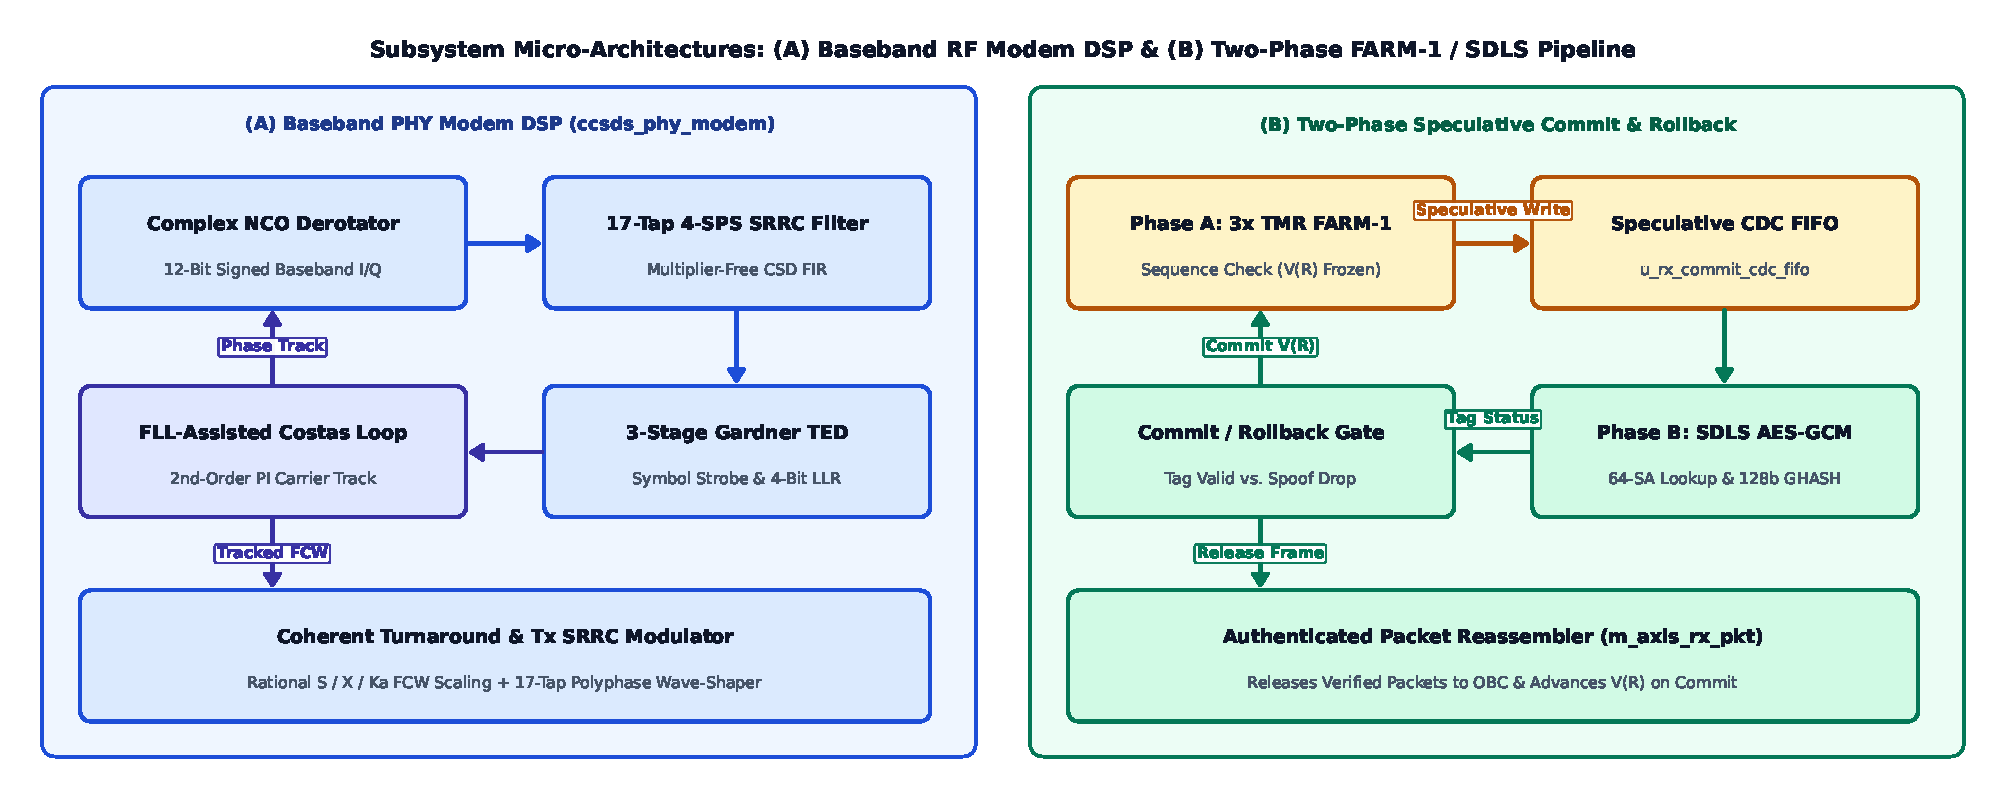
\includegraphics[width=0.95\textwidth]{docs/figures/fig2_phy_modem_and_two_phase_sdls.pdf}
    \vspace{-4pt}
    \caption{\small Baseband RF modem DSP pipeline (\texttt{ccsds\_phy\_modem.sv}) and Two-Phase \texttt{FARM-1}/\texttt{SDLS} commit/rollback architecture.}
\end{figure}

% =============================================================================
% CHAPTER 5: PROGRAMMER'S REGISTER MAP & BITFIELD REFERENCE (0x00-0x50)
% =============================================================================
\clearpage
\section{Programmer's Register Map (\texttt{0x00}--\texttt{0x50})}

All software interaction with \texttt{ccsds\_sat\_ttc\_top} takes place over the 32-bit AXI4-Lite slave interface (\texttt{rtl/ccsds\_axi\_lite\_csr.sv}). This chapter provides the complete address map from offset \texttt{0x00} through \texttt{0x50} (\textbf{Table~5.1}) followed by bit-by-bit field definitions for the mission configuration, timekeeping, fault telemetry, and SDLS cryptographic key/SA provisioning registers (\textbf{Tables~5.2--5.3}).

\subsection{Register Address Space Overview}
To protect mission configuration against radiation Single-Event Upsets (SEUs), all writable control registers (\texttt{0x04}, \texttt{0x08}, \texttt{0x0C}) are implemented as \textbf{3x Triple-Modular Redundant (TMR)} flip-flop banks (\texttt{*\_a\_q}, \texttt{*\_b\_q}, \texttt{*\_c\_q}) with continuous combinational majority voting and autonomous single-cycle SEU scrubbing.

\begin{table}[htbp]
\centering
\scriptsize
\renewcommand{\arraystretch}{1.15}
\begin{tabularx}{\textwidth}{@{}C{0.58in}L{1.45in}C{0.62in}C{0.82in}Y@{}}
\toprule
\textbf{Offset} & \textbf{Register Name} & \textbf{Access} & \textbf{Reset Value} & \textbf{Functional Summary} \\
\midrule
\texttt{0x00} & \texttt{CORE\_ID\_VER} & RO & \texttt{0xCC5D\_0230} & \texttt{[31:16]} Magic ID (\texttt{0xCC5D}), \texttt{[15:0]} Release Version (\texttt{0x0230}). \\
\texttt{0x04} & \texttt{CTRL\_SCID\_PROTO} & RW (3x TMR) & \texttt{0x0130\_0155} & Master protocol, downlink FEC, OCF/FECF, SDLS, SRRC, Gardner, and X$\to$Ka config (\textbf{Table~5.2}). \\
\texttt{0x08} & \texttt{CTRL\_USLP\_RS\_CFG} & RW (3x TMR) & \texttt{0x0001\_4255} & 16-bit USLP SCID, $\text{RS}(255,223)$ $(I,Q)$, \texttt{AES-128-GCM} mode, FLL assist, TM randomizer (\textbf{Table~5.3}). \\
\texttt{0x0C} & \texttt{CTRL\_COP1\_TFDF\_CFG} & RW (3x TMR) & \texttt{0x010D\_F010} & COP-1 sliding window half-width $W$, \texttt{TFDF} byte length, and Fault IRQ enable (\textbf{Table~5.3}). \\
\texttt{0x10} & \texttt{OBT\_COARSE\_SEC} & RW & \texttt{0x6530\_0000} & CCSDS 301.0-B-4 CUC On-Board Time 32-bit Coarse Seconds counter (\texttt{obt\_cuc\_48b[47:16]}). \\
\texttt{0x14} & \texttt{OBT\_FINE\_SUBSEC} & RW & \texttt{0x0000\_0000} & \texttt{[15:0]} CUC On-Board Time 16-bit Fine Sub-Seconds counter ($2^{-16}\,\text{s} = 15.26\,\mu\text{s}$ LSB). \\
\texttt{0x18} & \texttt{EDAC\_CORR\_CNTS} & RO / W1C & \texttt{0x0000\_0000} & \texttt{[15:0]} SECDED/BCH 1-bit corrected count (W1C bit 0); \texttt{[31:16]} 3x TMR SEU scrub count (W1C bit 16). \\
\texttt{0x1C} & \texttt{FAULT\_ERR\_CNTS} & RO / W1C & \texttt{0x0000\_0000} & \texttt{[15:0]} Uncorrectable FEC/CRC/Pkt error count (W1C bit 0); \texttt{[31:16]} SDLS MAC error count (W1C bit 16). \\
\texttt{0x20} & \texttt{LATEST\_CLCW\_MON} & RO & \texttt{0x0000\_0000} & Live 32-bit COP-1 \texttt{CLCW} monitor (\texttt{[7:0]} = $V(R)$, \texttt{[11]} = \texttt{Retransmit}, \texttt{[13]} = \texttt{Lockout}). \\
\texttt{0x24} & \texttt{LATEST\_PLCW\_MON} & RO & \texttt{0x0000\_0000} & Live 32-bit Proximity-1 COP-P \texttt{PLCW} monitor (\texttt{[7:0]} = $V(R)$ report value). \\
\texttt{0x28..0x44} & \texttt{REG\_SDLS\_KEY\_0..7} & RW & \texttt{0x1C1D..0203} & Eight 32-bit words forming the 256-bit SDLS Master Key (\texttt{0x28}=LSW \texttt{[31:0]} .. \texttt{0x44}=MSW \texttt{[255:224]}). \\
\texttt{0x48} & \texttt{REG\_SDLS\_SA\_CTRL} & RW & \texttt{0x0001\_0001} & \texttt{[15:0]} Default Tx SPI (\texttt{0x0001}); \texttt{[21:16]} SA RAM write address (\texttt{6'd1}); \texttt{[31]} Self-clearing SA write strobe. \\
\texttt{0x4C} & \texttt{REG\_SDLS\_SA\_SPI} & RW & \texttt{0x0000\_0001} & \texttt{[15:0]} 16-bit Security Parameter Index (\texttt{SPI}) to write into SA RAM entry \texttt{SA\_WR\_ADDR}. \\
\texttt{0x50} & \texttt{REG\_SDLS\_SA\_SEQ} & RW & \texttt{0x0000\_0000} & \texttt{[31:0]} Initial 32-bit Anti-Replay Sequence Number to write into SA RAM entry \texttt{SA\_WR\_ADDR}. \\
\bottomrule
\end{tabularx}
\caption{\footnotesize Complete AXI4-Lite Register Map (\texttt{0x00..0x50}) in \texttt{rtl/ccsds\_axi\_lite\_csr.sv}.}
\end{table}

\subsection{Control \& Security Register Bitfields}
\textbf{Table~5.2} and \textbf{Table~5.3} specify the individual bitfields of the primary control registers (\texttt{0x04}, \texttt{0x08}, \texttt{0x0C}) and the Security Association provisioning control register (\texttt{0x48}). Note how the hardware reset constant \texttt{RESET\_SCID\_PROTO = 32'h0131\_5155} in \texttt{rtl/ccsds\_axi\_lite\_csr.sv} decodes bit-for-bit in \textbf{Table~5.2}; at boot, flight software invokes \texttt{ccsds\_ttc\_hal\_configure()} to program validated mission protocol and FEC settings.

\begin{table}[htbp]
\centering
\scriptsize
\renewcommand{\arraystretch}{1.14}
\begin{tabularx}{\textwidth}{@{}C{0.62in}L{1.35in}C{0.55in}Y@{}}
\toprule
\textbf{Bits} & \textbf{Field Name} & \textbf{Reset} & \textbf{Register \texttt{0x04}: \texttt{CTRL\_SCID\_PROTO} (RW, 3x TMR, Reset \texttt{0x0130\_0155}) Description} \\
\midrule
\texttt{[31:30]} & \texttt{TURNAROUND\_KABAND} & \texttt{2'b00} & \texttt{00}: Use \texttt{turnaround\_xband\_cfg} strap (S-Band $240/221$ or X-Band $880/749$); \texttt{01}: X$\to$Ka Cross-Band Deep-Space Cat-B ($3344/749$); \texttt{10/11}: X$\to$Ka Cross-Band Near-Earth Cat-A ($3360/749$ / $3328/749$). \\
\texttt{[29]} & \texttt{GARDNER\_TED\_EN} & \texttt{1'b0} & \texttt{1}: Enables closed-loop 3-stage 4-SPS Gardner timing error detector (\texttt{SRRC\_4SPS\_EN} must be \texttt{1}). \\
\texttt{[28]} & \texttt{SRRC\_4SPS\_EN} & \texttt{1'b0} & \texttt{1}: Enables 17-tap CSD 4-SPS Square-Root Raised-Cosine ($\alpha=0.35$) Tx/Rx matched filters. \\
\texttt{[27]} & \texttt{BC\_REQ\_SDLS} & \texttt{1'b0} & \texttt{0}: Exempts COP-1 \texttt{Type-BC} (\texttt{Unlock}/\texttt{Set V(R)}) frames from SDLS per CCSDS 355.0-B-2 \S 3.3.2.3; \texttt{1}: Enforces SDLS on all frames. \\
\texttt{[26]} & \texttt{SDLS\_EN} & \texttt{1'b0} & \texttt{1}: Enables inline \texttt{ccsds\_sdls\_engine} encryption/authentication (OR-ed with \texttt{sdls\_en\_cfg} pin). \\
\texttt{[25]} & \texttt{OBT\_SEC\_HDR\_EN} & \texttt{1'b0} & \texttt{1}: Inserts 8-byte CCSDS 301.0-B-4 CUC On-Board Time Secondary Header into downlink TM frames. \\
\texttt{[24]} & \texttt{TC\_SEG\_HDR\_EN} & \texttt{1'b1} & \texttt{1}: Expects/generates the 8-bit TC Segment Header (\texttt{Seq\_Flags[1:0], MAP\_ID[5:0]}) in \texttt{PROTO\_TC}. \\
\texttt{[23]} & \texttt{AOS\_FHEC\_EN} & \texttt{1'b0} & \texttt{1}: Enables 16-bit $GF(2^4)$ $\text{RS}(10,6)$ Frame Header Error Control in \texttt{PROTO\_AOS} / \texttt{PROTO\_USLP}. \\
\texttt{[22]} & \texttt{FECF\_CRC32} & \texttt{1'b0} & \texttt{0}: 16-bit CRC-16-CCITT (\texttt{0x1021}); \texttt{1}: 32-bit Proximity-1/USLP CRC-32 (\texttt{0x00A00805}). \\
\texttt{[21]} & \texttt{FECF\_EN} & \texttt{1'b1} & \texttt{1}: Appends/verifies Frame Error Control Field (CRC-16/32) on all Transfer Frames. \\
\texttt{[20]} & \texttt{OCF\_EN} & \texttt{1'b1} & \texttt{1}: Appends 32-bit Operational Control Field (\texttt{CLCW} or \texttt{PLCW}) to downlink frames. \\
\texttt{[19:16]} & \texttt{FEC\_MODE} & \texttt{4'h0} & Downlink FEC select (\texttt{0}=Uncoded [default at reset], \texttt{1}=Reserved\_Uncoded, \texttt{4}=Conv $K=7$, \texttt{5}=$\text{RS}(255,223)$, \texttt{7}=Concat RS+Conv, \texttt{8}=AR4JA, \texttt{10..13}=Turbo). \\
\texttt{[14:12]} & \texttt{PROTO\_MODE} & \texttt{3'd0} & Active link protocol (\texttt{0}=TM default at reset, \texttt{1}=TC, \texttt{2}=AOS, \texttt{3}=Proximity-1, \texttt{4}=USLP). \\
\texttt{[15], [11:10]} & \texttt{RESERVED} & \texttt{3'b000} & Reserved bits, read as \texttt{0}. \\
\texttt{[9:0]} & \texttt{SCID\_10B} & \texttt{10'h155} & 10-bit Spacecraft Identifier for TM, TC, and Proximity-1 (lower 8 bits used for AOS). \\
\bottomrule
\end{tabularx}
\caption{\footnotesize Exact Bit-by-Bit Specification for Register \texttt{0x04} (\texttt{CTRL\_SCID\_PROTO}, Reset \texttt{0x0130\_0155}).}
\end{table}

\begin{table}[htbp]
\centering
\scriptsize
\renewcommand{\arraystretch}{1.14}
\begin{tabularx}{\textwidth}{@{}C{0.58in}C{0.62in}L{1.35in}C{0.58in}Y@{}}
\toprule
\textbf{Reg} & \textbf{Bits} & \textbf{Field Name} & \textbf{Reset} & \textbf{Registers \texttt{0x08}, \texttt{0x0C}, and \texttt{0x48..0x50} Bitfield Descriptions} \\
\midrule
\texttt{0x08} & \texttt{[30]} & \texttt{TM\_RAND\_EN\_CFG} & \texttt{1'b0} & \texttt{1}: Enables downlink CCSDS 131.0-B-5 $h_{\text{TM}}(x) = x^8+x^7+x^5+x^3+1$ CADU pseudo-randomizer. \\
\texttt{0x08} & \texttt{[29]} & \texttt{FLL\_ASSIST\_EN} & \texttt{1'b0} & \texttt{1}: Enables sign-quantized Differential Cross-Product FLL discriminator for wide-CFO pull-in ($\pm 640$ steps). \\
\texttt{0x08} & \texttt{[28]} & \texttt{SDLS\_GCM\_MODE} & \texttt{1'b0} & \texttt{0}: \texttt{AES-128-CTR} mode; \texttt{1}: Full NIST SP 800-38D \texttt{AES-128-GCM} with 128-bit $GF(2^{128})$ \texttt{GHASH} tag. \\
\texttt{0x08} & \texttt{[27:20]} & \texttt{RS\_VIRT\_FILL\_Q} & \texttt{8'd0} & Implicit virtual fill length $Q \in [0..200]$ bytes per $\text{RS}(255,223)$ codeword (shortens message to $223-Q$). \\
\texttt{0x08} & \texttt{[19:16]} & \texttt{RS\_INTERLEAVE\_I} & \texttt{4'd1} & Reed-Solomon interleaving depth $I \in \{1, 2, 3, 4, 5, 8\}$ codewords per CADU. \\
\texttt{0x08} & \texttt{[15:0]} & \texttt{USLP\_SCID\_16B} & \texttt{16'h4255} & 16-bit Spacecraft Identifier inserted into CCSDS 732.1-B-3 USLP Primary Headers. \\
\midrule
\texttt{0x0C} & \texttt{[24]} & \texttt{FAULT\_IRQ\_EN} & \texttt{1'b1} & \texttt{1}: Enables \texttt{fault\_irq\_out} assertion when \texttt{FAULT\_ERR\_CNTS} (\texttt{0x1C}) is non-zero. \\
\texttt{0x0C} & \texttt{[18:8]} & \texttt{TFDF\_BYTE\_LEN} & \texttt{11'd223} & Transfer Frame Data Field byte length ($\in [1..1024]$, set to $223 - Q - \text{Header/Trailer Overhead}$ for RS). \\
\texttt{0x0C} & \texttt{[7:0]} & \texttt{WINDOW\_HALF\_W} & \texttt{8'd16} & COP-1 \texttt{FARM-1} positive/negative sliding window half-width $W \in [1..128]$. \\
\midrule
\texttt{0x48} & \texttt{[31]} & \texttt{SA\_WR\_EN} & \texttt{1'b0} & Self-clearing write strobe: writing \texttt{1} commits \texttt{REG\_SDLS\_SA\_SPI} (\texttt{0x4C}) and \texttt{SEQ} (\texttt{0x50}) into SA RAM \texttt{[21:16]}. \\
\texttt{0x48} & \texttt{[21:16]} & \texttt{SA\_WR\_ADDR} & \texttt{6'd1} & Target 6-bit VCID / SA table index (\texttt{0..63}) in the Hsiao $(39,32)$ SECDED Security Association RAM. \\
\texttt{0x48} & \texttt{[15:0]} & \texttt{TX\_DEFAULT\_SPI} & \texttt{16'd1} & Default 16-bit Security Parameter Index (\texttt{SPI}) stamped into outgoing SDLS Security Headers. \\
\bottomrule
\end{tabularx}
\caption{\footnotesize Bitfield Specifications for \texttt{CTRL\_USLP\_RS\_CFG} (\texttt{0x08}), \texttt{CTRL\_COP1\_TFDF\_CFG} (\texttt{0x0C}), and \texttt{REG\_SDLS\_SA\_CTRL} (\texttt{0x48}).}
\end{table}

% =============================================================================
% CHAPTER 6: BARE-METAL ISO C11 HAL SDK & FLIGHT SOFTWARE INTEGRATION GUIDE
% =============================================================================
\vspace{6pt}
\section{Bare-Metal ISO C11 HAL SDK \& Software Recipes}

To eliminate error-prone manual bitmask manipulation in flight software, the repository includes a zero-dependency ISO C11 Hardware Abstraction Layer (\texttt{sw/ccsds\_ttc\_hal.h} and \texttt{sw/ccsds\_ttc\_hal.c}). Designed for safety-critical flight operating systems (RTEMS, FreeRTOS, NASA cFS, Zephyr) and bare-metal bootloaders on RISC-V, ARM Cortex-R, and LEON3/4 processors, the SDK requires only standard freestanding C headers (\texttt{<stdint.h>}, \texttt{<stdbool.h>}, \texttt{<stddef.h>}) and uses zero dynamic memory allocation. This chapter provides a detailed function-by-function API reference, explains the eight pre-commit CCSDS Blue Book configuration gating rules, and presents complete production flight software recipes.

\subsection{HAL API Function Reference (\texttt{sw/ccsds\_ttc\_hal.h})}
Each of the twelve public functions in \texttt{sw/ccsds\_ttc\_hal.h} is documented below in detail with its exact C prototype, parameter semantics, hardware register transactions, and return status codes.

\apifunc{int ccsds\_ttc\_hal\_init(ccsds\_ttc\_dev\_t *dev, volatile uint32\_t *base\_addr);}%
{Initializes a driver instance handle and verifies hardware presence on the AXI4-Lite bus before allowing any configuration writes.}%
{\texttt{dev} \emph{[out]}: Pointer to caller-allocated \texttt{ccsds\_ttc\_dev\_t} device context structure; \texttt{base\_addr} \emph{[in]}: Physical or virtual MMIO base address of \texttt{ccsds\_sat\_ttc\_top}.}%
{Performs a 32-bit volatile read from offset \texttt{0x00} (\texttt{CORE\_ID\_VER}) and checks that the returned word equals \texttt{0xCC5D0230UL} (\texttt{CCSDS\_EXPECTED\_VERSION\_ID}).}%
{\texttt{CCSDS\_HAL\_OK (0)} on success; \texttt{CCSDS\_HAL\_ERR\_NULL\_PTR (-1)} if \texttt{dev} or \texttt{base\_addr} is \texttt{NULL}; \texttt{CCSDS\_HAL\_ERR\_BAD\_VERSION (-2)} if the hardware version register does not match \texttt{0xCC5D0230UL}.}

\apifunc{int ccsds\_ttc\_hal\_validate\_config(const ccsds\_ttc\_config\_t *cfg);}%
{Audits a candidate transceiver configuration structure against all eight cross-layer CCSDS Blue Book compatibility rules in software without touching hardware registers.}%
{\texttt{cfg} \emph{[in]}: Pointer to a populated \texttt{ccsds\_ttc\_config\_t} configuration structure.}%
{Pure software validation function; performs zero MMIO reads or writes. Used both standalone and as the pre-commit gate inside \texttt{ccsds\_ttc\_hal\_configure()}.}%
{\texttt{CCSDS\_HAL\_OK (0)} if valid, or a specific negative error code (\texttt{-1} or \texttt{-10..-17}; see Subsection~6.2) identifying the exact CCSDS rule violation.}

\apifunc{int ccsds\_ttc\_hal\_configure(const ccsds\_ttc\_dev\_t *dev, const ccsds\_ttc\_config\_t *cfg);}%
{Validates and atomically commits a complete protocol, FEC, PHY, COP-1, and SDLS configuration to the 3x TMR hardware control registers.}%
{\texttt{dev} \emph{[in]}: Initialized device handle; \texttt{cfg} \emph{[in]}: Desired transceiver configuration structure.}%
{First calls \texttt{ccsds\_ttc\_hal\_validate\_config(cfg)}. If and only if validation returns \texttt{0}, packs the bitfields and writes \texttt{0x04} (\texttt{CTRL\_SCID\_PROTO}), \texttt{0x08} (\texttt{CTRL\_USLP\_RS\_CFG}), and \texttt{0x0C} (\texttt{CTRL\_COP1\_TFDF\_CFG}). If validation fails, hardware registers remain untouched.}%
{\texttt{CCSDS\_HAL\_OK (0)} on commit, or the negative validation error code (\texttt{-1}, \texttt{-10..-17}).}

\apifunc{void ccsds\_ttc\_hal\_get\_config(const ccsds\_ttc\_dev\_t *dev, ccsds\_ttc\_config\_t *cfg\_out);}%
{Reads back the currently active 3x TMR voted configuration registers from hardware and unpacks them into a C structure for telemetry verification or state auditing.}%
{\texttt{dev} \emph{[in]}: Initialized device handle; \texttt{cfg\_out} \emph{[out]}: Destination structure populated with active hardware settings.}%
{Executes three 32-bit reads from offsets \texttt{0x04}, \texttt{0x08}, and \texttt{0x0C} (which return the combinational majority-voted output of the triplicated TMR banks).}%
{\texttt{void} (no-op if either pointer is \texttt{NULL}).}

\apifunc{int ccsds\_ttc\_hal\_set\_sdls\_key256(const ccsds\_ttc\_dev\_t *dev, const uint32\_t key\_words[8]);}%
{Loads a 128-bit or 256-bit cryptographic Master Key into the SDLS engine for \texttt{AES-128-CTR} and \texttt{AES-128-GCM} authenticated encryption and decryption.}%
{\texttt{dev} \emph{[in]}: Initialized device handle; \texttt{key\_words[8]} \emph{[in]}: Array of eight 32-bit words (\texttt{key\_words[0]} = LSW \texttt{[31:0]} through \texttt{key\_words[7]} = MSW \texttt{[255:224]}).}%
{Writes offsets \texttt{0x28}, \texttt{0x2C}, \texttt{0x30}, \texttt{0x34}, \texttt{0x38}, \texttt{0x3C}, \texttt{0x40}, and \texttt{0x44} (\texttt{REG\_SDLS\_KEY\_0..7}).}%
{\texttt{CCSDS\_HAL\_OK (0)} on success; \texttt{CCSDS\_HAL\_ERR\_NULL\_PTR (-1)} if either pointer is \texttt{NULL}.}

\apifunc{int ccsds\_ttc\_hal\_provision\_sdls\_sa(const ccsds\_ttc\_dev\_t *dev, uint8\_t vcid\_addr, uint16\_t spi, uint32\_t seq\_low, uint16\_t tx\_default\_spi);}%
{Provisions an entry in the 64-entry Hsiao $(39,32)$ SECDED-protected Security Association (SA) RAM for a specific Virtual Channel (\texttt{vcid\_addr}) and sets the default transmit \texttt{SPI}. To prevent GCM IV reuse across Virtual Channels or spacecraft, set \texttt{spi = (scid\_10b << 6) | vcid\_addr}.}%
{\texttt{dev} \emph{[in]}: Device handle; \texttt{vcid\_addr} \emph{[in]}: SA table index (\texttt{0..63}); \texttt{spi} \emph{[in]}: Expected 16-bit Security Parameter Index; \texttt{seq\_low} \emph{[in]}: Initial 32-bit anti-replay sequence number threshold; \texttt{tx\_default\_spi} \emph{[in]}: 16-bit \texttt{SPI} stamped on outgoing downlink frames.}%
{Writes \texttt{spi} to \texttt{0x4C} (\texttt{REG\_SDLS\_SA\_SPI}), writes \texttt{seq\_low} to \texttt{0x50} (\texttt{REG\_SDLS\_SA\_SEQ}), and writes \texttt{(1U << 31) | ((vcid\_addr \& 0x3FU) << 16) | tx\_default\_spi} to \texttt{0x48} (\texttt{REG\_SDLS\_SA\_CTRL}), triggering a single-cycle Hsiao SECDED-encoded write into SA RAM.}%
{\texttt{CCSDS\_HAL\_OK (0)} on success; \texttt{-1} if \texttt{dev == NULL} or \texttt{vcid\_addr > 63}.}

\apifunc{void ccsds\_ttc\_hal\_get\_clcw(const ccsds\_ttc\_dev\_t *dev, ccsds\_clcw\_status\_t *clcw\_out);}%
{Reads the latest 32-bit COP-1 Communications Link Control Word (\texttt{CLCW}) and unpacks all status flags and the receiver sequence counter $V(R)$.}%
{\texttt{dev} \emph{[in]}: Device handle; \texttt{clcw\_out} \emph{[out]}: Pointer to \texttt{ccsds\_clcw\_status\_t} receiving \texttt{vcid}, \texttt{no\_rf\_avail}, \texttt{no\_bit\_lock}, \texttt{lockout}, \texttt{wait\_flag}, \texttt{retransmit}, \texttt{farm\_b\_counter}, and \texttt{report\_value} ($V(R)$).}%
{Reads offset \texttt{0x20} (\texttt{LATEST\_CLCW\_MON}). On Spacecraft (\texttt{ROLE=0}), reflects local \texttt{FARM-1} state; on Ground EGSE (\texttt{ROLE=1}), reflects the latest \texttt{CLCW} extracted from downlink telemetry.}%
{\texttt{void}.}

\apifunc{uint64\_t ccsds\_ttc\_hal\_get\_obt\_cuc48(const ccsds\_ttc\_dev\_t *dev);\newline void ccsds\_ttc\_hal\_set\_obt\_cuc48(const ccsds\_ttc\_dev\_t *dev, uint32\_t coarse\_sec, uint16\_t fine\_subsec);}%
{Reads or initializes the 48-bit CCSDS 301.0-B-4 Unsegmented Time Code (\texttt{OBT}) counter ($32$-bit coarse seconds in bits \texttt{[47:16]} and $16$-bit fine sub-seconds in bits \texttt{[15:0]}).}%
{\texttt{dev} \emph{[in]}: Device handle; \texttt{coarse\_sec} \emph{[in]}: 32-bit seconds epoch; \texttt{fine\_subsec} \emph{[in]}: 16-bit fractional seconds ($2^{-16}\,\text{s}$ LSB).}%
{Accesses offsets \texttt{0x10} (\texttt{OBT\_COARSE\_SEC}) and \texttt{0x14} (\texttt{OBT\_FINE\_SUBSEC}).}%
{\texttt{get\_obt\_cuc48} returns the packed 48-bit timestamp in a \texttt{uint64\_t}; \texttt{set\_obt\_cuc48} returns \texttt{void}.}

\apifunc{void ccsds\_ttc\_hal\_get\_error\_telemetry(const ccsds\_ttc\_dev\_t *dev, ccsds\_err\_telemetry\_t *err\_out);\newline void ccsds\_ttc\_hal\_clear\_error\_telemetry(const ccsds\_ttc\_dev\_t *dev, bool clr\_edac, bool clr\_tmr, bool clr\_uncorr, bool clr\_sdls);}%
{Reads or selectively clears the four saturating 16-bit hardware EDAC, TMR SEU, uncorrectable FEC/CRC, and SDLS MAC authentication error counters.}%
{\texttt{dev} \emph{[in]}: Device handle; \texttt{err\_out} \emph{[out]}: Structure receiving all 4 counters; \texttt{clr\_*} \emph{[in]}: Booleans selecting which counters to clear via Write-1-to-Clear (W1C).}%
{Reads or writes W1C strobes (\texttt{bit 0} and \texttt{bit 16}) to offsets \texttt{0x18} (\texttt{EDAC\_CORR\_CNTS}) and \texttt{0x1C} (\texttt{FAULT\_ERR\_CNTS}).}%
{\texttt{void}.}

\apifunc{uint32\_t ccsds\_ttc\_hal\_reg\_read(const ccsds\_ttc\_dev\_t *dev, uint32\_t reg\_offset);\newline void ccsds\_ttc\_hal\_reg\_write(const ccsds\_ttc\_dev\_t *dev, uint32\_t reg\_offset, uint32\_t val);}%
{Low-level volatile 32-bit MMIO register read and write primitives for custom diagnostic or register-test routines.}%
{\texttt{dev} \emph{[in]}: Device handle; \texttt{reg\_offset} \emph{[in]}: Byte offset (\texttt{0x00..0x50}); \texttt{val} \emph{[in]}: 32-bit word to write.}%
{Directly dereferences \texttt{dev->base\_addr + (reg\_offset >> 2)}.}%
{\texttt{reg\_read} returns the 32-bit register value; \texttt{reg\_write} returns \texttt{void}.}

\subsection{Pre-Commit Configuration Gating Rules}
To prevent flight software from accidentally programming an illegal combination of modulation, line coding, framing protocol, and FEC codec, \texttt{ccsds\_ttc\_hal\_validate\_config()} enforces eight cross-layer compatibility rules prior to any CSR write:
\begin{enumerate}\setlength{\itemsep}{2pt}
    \item \textbf{Modulation vs.\ Manchester Line Coding (\texttt{CCSDS\_HAL\_ERR\_MOD\_LINE\_INCOMPAT = -10}):} Per CCSDS 401.0-B-32 \cite{ccsds401}, split-phase Manchester (\texttt{Bi-$\phi$-L}) coding is only permitted with single-dimension carrier modulations (\texttt{BPSK} and residual-carrier \texttt{PCM/PSK/PM}). Pairing \texttt{QPSK} or \texttt{OQPSK} with \texttt{Bi-$\phi$-L} is rejected (leaving 10 valid modulation $\times$ line-code waveform pairs).
    \item \textbf{4-SPS SRRC Pulse Shaping vs.\ Manchester Coding (\texttt{CCSDS\_HAL\_ERR\_SRRC\_BIPHI\_INCOMPAT = -11}):} Square-Root Raised-Cosine (\texttt{srrc\_4sps\_en = 1}) matched filtering is defined strictly for baseband \texttt{NRZ-L} and \texttt{NRZ-M} pulses; enabling SRRC alongside \texttt{Bi-$\phi$-L} distorts the mid-bit Manchester transition and is rejected.
    \item \textbf{4-SPS Gardner Timing Recovery Dependency (\texttt{CCSDS\_HAL\_ERR\_GARDNER\_REQUIRES\_4SPS = -12}):} The Gardner Timing Error Detector (\texttt{gardner\_ted\_en = 1}) requires 4 samples per symbol from the SRRC matched filter (\texttt{srrc\_4sps\_en = 1}); enabling Gardner TED with \texttt{srrc\_4sps\_en = 0} is rejected.
    \item \textbf{Protocol vs.\ Directional FEC Compatibility (\texttt{CCSDS\_HAL\_ERR\_PROTO\_FEC\_INCOMPAT = -13}):} Rejects pairing Uplink-only Telecommand (\texttt{PROTO\_TC}) with Downlink-only codecs ($\text{RS}(255,223)$, Turbo, AR4JA), rejects pairing Downlink-only \texttt{PROTO\_TM}/\texttt{AOS} with Uplink-only codecs ($\text{BCH}(63,56)$, Short-LDPC), and restricts \texttt{PROTO\_PROX1} to uncoded or $K=7$ convolutional coding per CCSDS 211.2-B-3.
    \item \textbf{CRC-16 vs.\ CRC-32 FECF Mandate (\texttt{CCSDS\_HAL\_ERR\_CRC32\_PROTO\_INCOMPAT = -14}):} Enforces 16-bit CRC-16 (\texttt{fecf\_crc32 = 0}) on \texttt{TM}, \texttt{AOS}, and \texttt{TC}, mandates 32-bit CRC-32 (\texttt{fecf\_crc32 = 1}) on \texttt{Proximity-1}, and allows either CRC-16 or CRC-32 on \texttt{USLP}.
    \item \textbf{AOS Frame Header Error Control Scope (\texttt{CCSDS\_HAL\_ERR\_AOS\_FHEC\_INCOMPAT = -15}):} Rejects enabling the 16-bit $GF(2^4)$ $\text{RS}(10,6)$ \texttt{FHEC} (\texttt{aos\_fhec\_en = 1}) unless the active protocol is \texttt{PROTO\_AOS} or \texttt{PROTO\_USLP}.
    \item \textbf{Reed-Solomon Parameter Bounds (\texttt{CCSDS\_HAL\_ERR\_RS\_PARAM\_RANGE = -16}):} Enforces CCSDS 131.0-B-5 interleaving depth $I \in \{1, 2, 3, 4, 5, 8\}$ and virtual fill length $Q \le 215$.
    \item \textbf{Frame Length \& COP-1 Window Bounds (\texttt{CCSDS\_HAL\_ERR\_FRAME\_LEN\_RANGE = -17}):} Enforces $\text{TFDF\_BYTE\_LEN} \in [1..1024]$, verifies that total Transfer Frame size ($\text{TFDF\_BYTE\_LEN} + \text{Header/OCF/FECF/SDLS Overhead}$) does not exceed $223 - Q$ bytes when $\text{RS}(255,223)$ ($I=1$) is active, and enforces COP-1 sliding window half-width $W \in [1..128]$.
\end{enumerate}

\subsection{Flight Software Integration Recipes}
When configuring $\text{RS}(255,223)$ ($I=1, Q=0$), each codeword carries exactly $223\text{ bytes}$ of total Transfer Frame data. With TM Primary Header ($6\text{ B}$) + CUC OBT Secondary Header ($8\text{ B}$) + SDLS Security Header ($6\text{ B}$) + SDLS AES-128-GCM Tag ($16\text{ B}$) + CLCW OCF ($4\text{ B}$) + CRC-16 FECF ($2\text{ B}$) $= \mathbf{42\text{ bytes}}$ of framing and security overhead, \texttt{.tfdf\_byte\_len} is configured to $223 - 42 = \mathbf{181\text{ bytes}}$ (\texttt{181U}) so each Transfer Frame maps 1:1 into a 255-byte Reed-Solomon CADU:

\begin{lstlisting}[language=C,style=ccode]
#include "ccsds_ttc_hal.h"

/* Recipe 1: Spacecraft Flight Boot, Domain-Separated SDLS Key/SA Load & 223B RS Frame Config */
int spacecraft_ttc_boot_init(ccsds_ttc_dev_t *dev, volatile uint32_t *mmio_base) {
    int status = ccsds_ttc_hal_init(dev, mmio_base);
    if (status != CCSDS_HAL_OK) return status;

    /* 1. Load 128-bit/256-bit Master Key into 0x28..0x44 and provision VCID=0..7 with domain-separated
     *    SPI = (SCID_10B << 6) | VCID so no two Virtual Channels or spacecraft ever reuse a GCM IV */
    const uint32_t mission_key[8] = {
        0x3C4FCF09UL, 0x8815F7ABUL, 0xA6D2AE28UL, 0x16157E2BUL,
        0x00000000UL, 0x00000000UL, 0x00000000UL, 0x00000000UL
    };
    const uint16_t scid_10b = 0x0155U;
    const uint16_t default_spi = (uint16_t)((scid_10b << 6) | 0U); /* 0x5540 for SCID=0x155, VCID=0 */
    ccsds_ttc_hal_set_sdls_key256(dev, mission_key);
    for (uint8_t vcid = 0U; vcid < 8U; vcid++) {
        uint16_t vc_spi = (uint16_t)((scid_10b << 6) | vcid);
        ccsds_ttc_hal_provision_sdls_sa(dev, vcid, vc_spi, 0x00000000UL, default_spi);
    }

    /* 2. Configure Downlink TM + Concatenated RS(255,223)/Viterbi + 4-SPS SRRC/Gardner + AES-GCM.
     *    Total RS(255,223) info capacity = 223 B. Overhead = 6B(TM) + 8B(OBT) + 6B(SDLS Hdr)
     *    + 16B(GCM Tag) + 4B(OCF) + 2B(CRC16) = 42 B -> usable tfdf_byte_len = 223 - 42 = 181 B. */
    ccsds_ttc_config_t cfg = {
        .scid_10b           = scid_10b,
        .uslp_scid_16b      = 0x4255U,
        .proto_mode         = CCSDS_PROTO_TM,
        .fec_mode           = CCSDS_FEC_CONCAT_RS_CNV,
        .mod_mode           = CCSDS_MOD_QPSK,
        .line_code          = CCSDS_LINE_NRZ_L,
        .ocf_en             = true,   /* +4 B: Embed live 32-bit COP-1 CLCW in Downlink TM OCF */
        .fecf_en            = true,   /* +2 B: Append 16-bit CRC-16-CCITT FECF */
        .fecf_crc32         = false,
        .aos_fhec_en        = false,
        .tc_seg_hdr_present = true,
        .obt_sec_hdr_en     = true,   /* +8 B: Stamp 48-bit CUC On-Board Time Secondary Header */
        .sdls_en            = true,   /* +6 B Header + 16 B GCM Tag: Inline CCSDS 355.0-B-2 SDLS */
        .bc_require_sdls    = false,  /* Allow Type-BC Unlock recovery per 355.0-B-2 3.3.2.3 */
        .window_half_w      = 16U,
        .rs_interleave_i    = 1U,
        .rs_virt_fill_q     = 0U,
        .tfdf_byte_len      = 181U,   /* 181 B TFDF + 42 B Overhead = 223 B exact RS(255,223) block */
        .turnaround_kaband  = CCSDS_KABAND_NONE_OR_SX, /* S-Band 240/221 via strap */
        .srrc_4sps_en       = true,
        .gardner_ted_en     = true,
        .sdls_gcm_mode      = true,   /* Full 128-bit GHASH authenticated encryption */
        .fll_assist_en      = true,
        .tm_rand_en         = true,
        .fault_irq_en       = true
    };
    return ccsds_ttc_hal_configure(dev, &cfg);
}

/* Recipe 2: Periodic 1 Hz OBC Health ISR --- Poll CLCW, OBT & Scrub EDAC/TMR Counters */
void spacecraft_ttc_1hz_health_isr(const ccsds_ttc_dev_t *dev, ccsds_clcw_status_t *clcw,
                                   ccsds_err_telemetry_t *err, uint64_t *obt_cuc48) {
    *obt_cuc48 = ccsds_ttc_hal_get_obt_cuc48(dev);
    ccsds_ttc_hal_get_clcw(dev, clcw);
    ccsds_ttc_hal_get_error_telemetry(dev, err);

    if (err->secded_bch_single_corr_cnt || err->tmr_seu_corrected_cnt ||
        err->uncorr_frame_pkt_err_cnt   || err->sdls_mac_err_cnt) {
        ccsds_ttc_hal_clear_error_telemetry(dev, true, true, true, true);
    }
}
\end{lstlisting}

% =============================================================================
% CHAPTER 7: S-BAND BOARD INTEGRATION, WIRING & HARDWARE BRING-UP GUIDE
% =============================================================================
\newpage
\section{S-Band Board Integration, Wiring \& Bring-Up}

While \textbf{Volume~II, Chapter~7} derives the S-Band RF cascade, Friis noise-temperature equations, $600\,\text{km}$ LEO link budgets, and space-qualification rules from first principles, this chapter provides the practical \textbf{board-level hardware partitioning, pin wiring, and component bill of materials} for integrating the FPGA with an external SDR transceiver and S-Band RF Front-End (RFFE).

\subsection{Three-Subsystem Hardware Partitioning}
The reference S-Band full-duplex transceiver ($2025\text{--}2110\,\text{MHz}$ Uplink Rx / $2200\text{--}2290\,\text{MHz}$ Downlink Tx) partitions hardware across three physical subsystems (\textbf{Figure~7.1}):
\begin{enumerate}\setlength{\itemsep}{1.5pt}
    \item \textbf{Subsystem~1 --- Digital Baseband FPGA:} Hosts \texttt{ccsds\_sat\_ttc\_top}, the 16-bit LVDS Source-Synchronous Interface (\texttt{SSI}) bridge, the 4-wire SPI controller, and the $<500\,\text{ns}$ hardware PA enable latch.
    \item \textbf{Subsystem~2 --- Agile Zero-IF SDR \& Clock/PMIC Tree:} Performs direct quadrature RF conversion, closed-loop Digital Pre-Distortion (\texttt{DPD}), and phase-coherent $38.40\,\text{MHz}$ clock distribution.
    \item \textbf{Subsystem~3 --- S-Band Full-Duplex RFFE:} Provides pre-PA spectral filtering, $4\,\text{W}$ linear power amplification, reverse-power isolation, forward/reflected directional coupling, full-duplex diplexing, and ultra-low-noise receive amplification.
\end{enumerate}
Board-level wiring and zone-by-zone schematic connections are detailed in Section~7.2, followed by component selection and vacuum-derated operating modes in Section~7.3.

\begin{figure}[htbp]
    \centering
    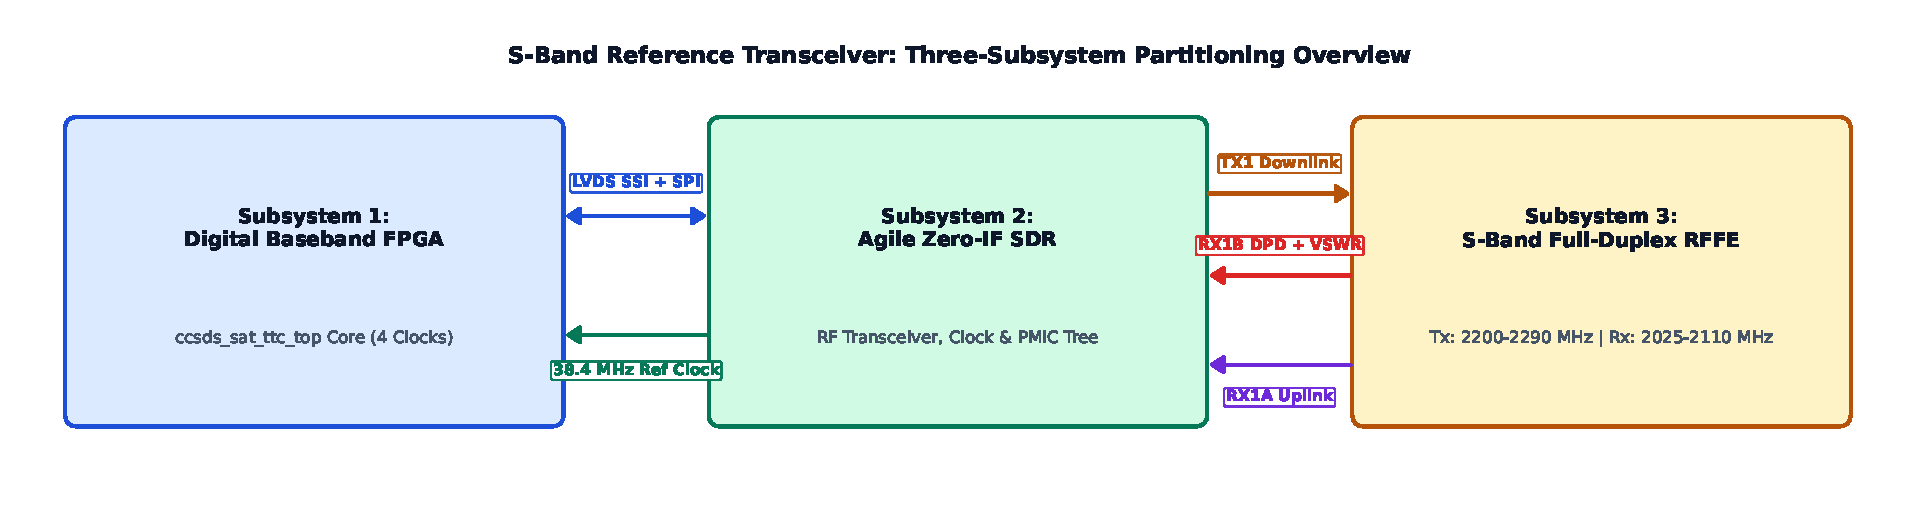
\includegraphics[width=0.92\textwidth]{docs/figures/fig_sband_3block_overview.pdf}
    \vspace{-4pt}
    \caption{\small Three-subsystem hardware partitioning of the S-Band full-duplex reference transceiver.}
\end{figure}

\subsection{Baseband-to-RF Interconnects \& PA Protection}
\textbf{Figure~7.2} presents the inter-zone signal connectivity overview (top panel) followed by four focused zone sub-diagrams (\textbf{Figures~7.2a--d}), and \textbf{Table~7.1} lists the exact board-level pin routing and termination rules. Quantitative RF cascade placement proofs are derived in \textbf{Volume~II, Section~7.1}; for board layout and bring-up, note three essential wiring rules in \textbf{Figure~7.2c}:
\begin{itemize}\setlength{\itemsep}{1.5pt}
    \item \textbf{Upstream RF Isolator (\texttt{\#3}) Before Bi-Directional Coupler (\texttt{\#2}):} Output RF Isolator \texttt{\#3} sits directly at the \texttt{SKY66294-11} PA output, while $20\,\text{dB}$ Bi-Directional Coupler \texttt{\#2} sits downstream between the Isolator and Diplexer \texttt{\#4}. This ordering allows Coupler Port~4 to sense true antenna reflections before the isolator's $20\,\text{W}$ termination load absorbs the reverse wave.
    \item \textbf{Sub-$500\,\text{ns}$ Hardware PA Cutoff (\texttt{\#8}):} Coupler Port~4 feeds the \href{https://www.analog.com/media/en/technical-documentation/data-sheets/ad8362.pdf}{\textbf{Analog Devices \texttt{AD8362}}} True-RMS detector, whose output splits to (a) a \textbf{TI \texttt{TLV4041R1}} comparator ($V_{\text{th}} = 1.15\,\text{V}$ for $\text{VSWR} = 3.0:1$) that asynchronously clears the FPGA \texttt{PA\_EN\_LATCH} in $<500\,\text{ns}$, and (b) \texttt{ADRV9002} \texttt{AUXADC\_0} for continuous pass telemetry.
    \item \textbf{Closed-Loop DPD Observation (\texttt{\#7A}):} Coupler Port~3 (forward coupled, $-20\,\text{dB}$) passes through a $30\,\text{dB}$ pad (\texttt{YAT-30A+}) into the \texttt{TCM2-33WX+} balun (\texttt{T203}) driving \texttt{ADRV9002} \texttt{RX1B}.
\end{itemize}

\begin{figure}[htbp]
    \centering
    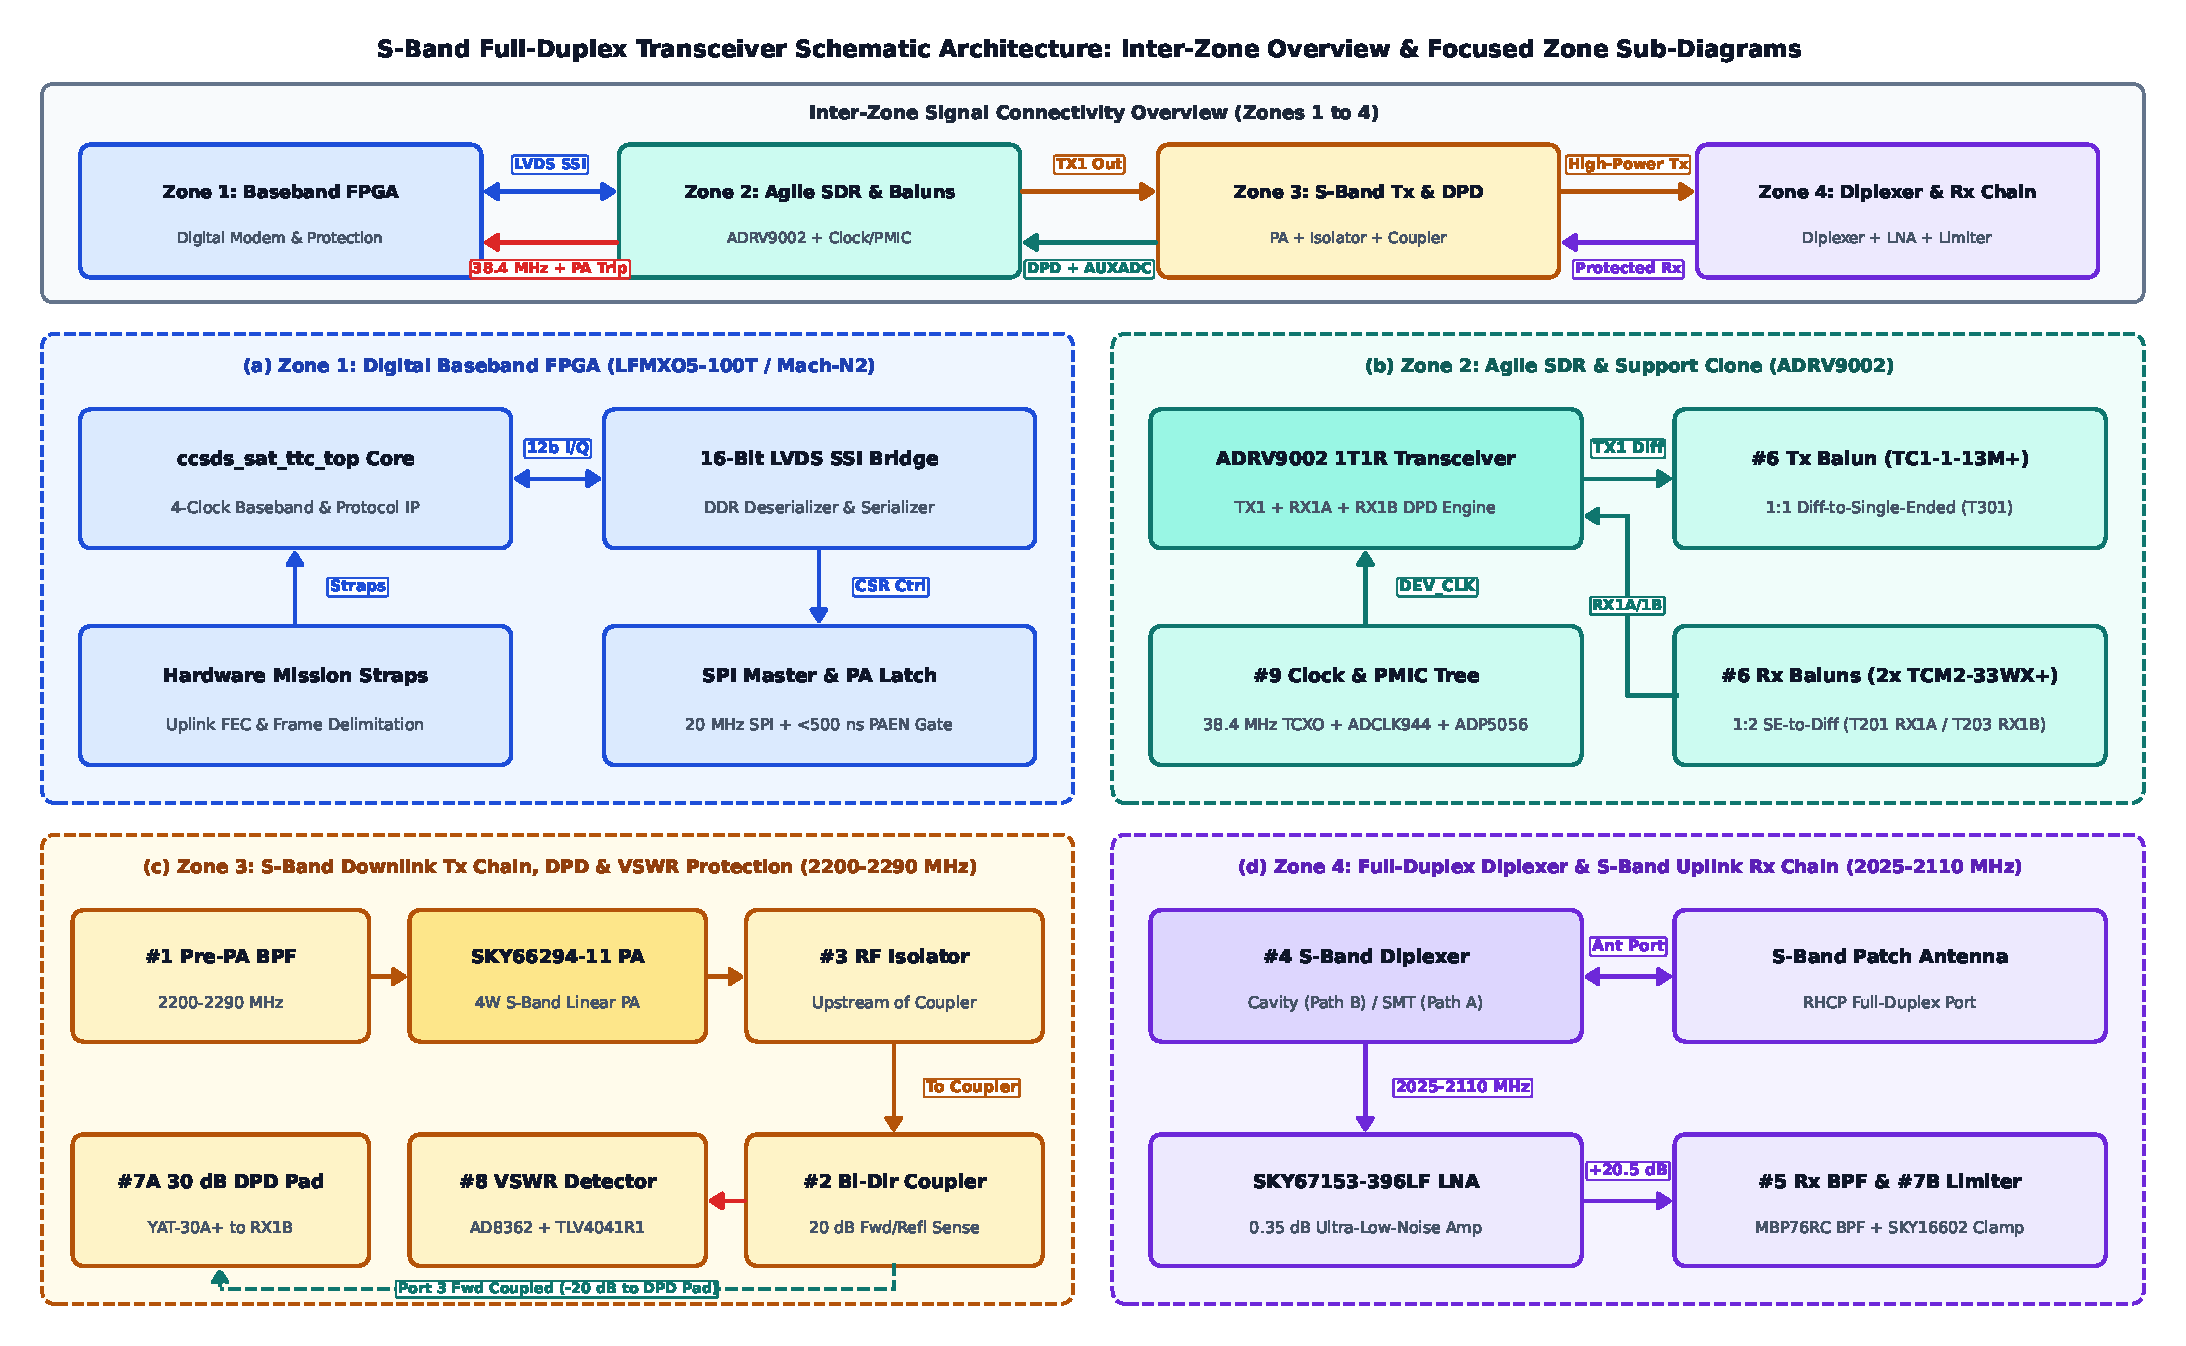
\includegraphics[width=1.00\textwidth]{docs/figures/fig4_sband_rffe_architecture.pdf}
    \vspace{-4pt}
    \caption{\small S-Band transceiver inter-zone connectivity overview and focused zone sub-diagrams (\texttt{a}--\texttt{d}).}
\end{figure}

\begin{table}[htbp]
\centering
\scriptsize
\renewcommand{\arraystretch}{1.14}
\begin{tabularx}{\textwidth}{@{}L{1.32in}L{1.28in}C{0.78in}Y@{}}
\toprule
\textbf{Signal Group} & \textbf{Board Net Name(s)} & \textbf{I/O Standard} & \textbf{Pin Routing \& Termination Requirement} \\
\midrule
\textbf{Master Reference Clock} & \texttt{DEV\_CLK\_IN$\pm$}, \texttt{FPGA\_REF\_CLK$\pm$} & LVPECL / LVDS ($100\,\Omega$) & Phase-synchronous $38.40\,\text{MHz}$ fanout from \texttt{ADCLK944BCPZ} (\texttt{U501}) fed by \texttt{GTXO-74V/JI} TCXO (\texttt{Y501}). \\
\textbf{Rx1A Baseband LVDS SSI} & \texttt{RX1\_DCLK$\pm$}, \texttt{RX1\_STROBE$\pm$}, \texttt{RX1\_IDATA$\pm$}, \texttt{RX1\_QDATA$\pm$} & $1.8\,\text{V}$ LVDS ($100\,\Omega$) & DDR LVDS from \texttt{ADRV9002} to FPGA Bank~2; deserializes 16-bit words and slices MSB \texttt{[15:4]} into \texttt{rx\_i/q\_adc\_in[11:0]}. \\
\textbf{Tx1 Baseband LVDS SSI} & \texttt{TX1\_DCLK$\pm$}, \texttt{RX1\_STROBE$\pm$}, \texttt{TX1\_IDATA$\pm$}, \texttt{TX1\_QDATA$\pm$} & $1.8\,\text{V}$ LVDS ($100\,\Omega$) & DDR LVDS from FPGA to \texttt{ADRV9002}; pads 12-bit \texttt{phy\_tx\_12b} as \texttt{\{phy\_tx\_12b, 4'b0000\}} into \texttt{[15:0]}. \\
\textbf{4-Wire Control SPI} & \texttt{SPI\_CLK}, \texttt{SPI\_CSB}, \texttt{SPI\_MOSI}, \texttt{SPI\_MISO} & $1.8\,\text{V}$ LVCMOS & $20\,\text{MHz}$ SPI bus from FPGA SPI Master to \texttt{ADRV9002} for boot init, $0.05\,\text{dB}$ Tx attenuation, and \texttt{AUXADC\_0} readback. \\
\textbf{Fast PA Enable \& VSWR Trip} & \texttt{PA\_FAULT\_COMP\_N} $\rightarrow$ \texttt{SKY\_PAEN} & $1.8\,\text{V} / 3.3\,\text{V}$ LVCMOS & Open-drain \texttt{TLV4041R1} comparator output from \texttt{AD8362}; pulls \texttt{SKY66294-11} \texttt{PAEN} low in $<500\,\text{ns}$ on $\text{VSWR} > 3:1$. \\
\bottomrule
\end{tabularx}
\caption{\footnotesize Board-level digital, clock, and PA protection interconnects between Zone~1, Zone~2, and Zone~3.}
\end{table}

\subsection{S-Band Bill of Materials \& Operating Modes}
The Flight PCB supports two passive filter assembly options: \textbf{Flight Path~B} uses a $20\,\text{W}$-rated combline cavity diplexer (\texttt{D0421552}) operated at full $+34.0\,\text{dBm}$ ($2.51\,\text{W}$) PA output, whereas \textbf{Flight Path~A} uses a compact all-SMT $3.0\,\text{W}$-rated ceramic diplexer (\texttt{CTS UPD215A}) operated at a \textbf{NASA EEE-INST-002 / ECSS-Q-ST-30-11C 50\% vacuum-derated $+31.5\,\text{dBm}$ ($1.41\,\text{W}$) PA output}. For rapid reference, the bill of materials is split into the \textbf{Downlink Transmit \& Protection Chain (\textbf{Table~7.2})} and the \textbf{Diplexer \& Uplink Receive Chain (\textbf{Table~7.3})}.

\begin{table}[htbp]
\centering
\scriptsize
\renewcommand{\arraystretch}{1.12}
\begin{tabularx}{\textwidth}{@{}L{0.92in}L{1.38in}L{1.72in}L{1.18in}Y@{}}
\toprule
\textbf{Tx / Core Stage} & \textbf{Stage Function} & \textbf{Flight PCB Part (Path B / Path A)} & \textbf{PoC Bench Setup} & \textbf{Operating Level (Path B / Path A)} \\
\midrule
\textbf{Core 1 + \#9} & FPGA + $38.4\,\text{MHz}$ Clock & \texttt{LFMXO5-100T} + \texttt{GTXO-74V} + \texttt{ADCLK944} & \texttt{LN2-MH-20-EVN} + \texttt{EVAL} & SEL-immune FD-SOI FPGA + \texttt{EVAL} clock/PMIC tree. \\
\textbf{Core 2 + \#6 Tx} & SDR + \texttt{TX1} $1:1$ Balun & \texttt{ADRV9002} + \texttt{TC1-1-13M+} (\texttt{T301}) & On \texttt{EVAL-ADRV9002} & $-1.7\,\text{dBm}$ (Path~B) / $-3.4\,\text{dBm}$ (Path~A) out of \texttt{T301}. \\
\textbf{Tx Stage 2 (\texttt{\#1})} & Pre-PA Tx Bandpass & \textbf{B}: \texttt{AE2250B10113} / \textbf{A}: \texttt{BFCN-2275+} & \texttt{TB-270} (\texttt{BFCN-2275+}) & Strips Rx-band DAC noise; $-2.5\,\text{dBm}$ (B) / $-5.0\,\text{dBm}$ (A). \\
\textbf{Tx Stage 3 (\texttt{PA})} & S-Band 4W Linear PA & \texttt{Skyworks SKY66294-11} ($+36.5\,\text{dB}$) & \texttt{SKY66294-11-EVB} & $+34.0\,\text{dBm}$ ($2.51\,\text{W}$ B) / $+31.5\,\text{dBm}$ ($1.41\,\text{W}$ A, derated). \\
\textbf{Tx Stage 4 (\texttt{\#3})} & Output RF Isolator & \textbf{B}: \texttt{RFCI RFSL2848} / \textbf{A}: \texttt{RFCR2848S} & \texttt{RFCI RFSL3818} (SMA) & Upstream of coupler; $+33.80\,\text{dBm}$ (B) / $+31.25\,\text{dBm}$ (A). \\
\textbf{Tx Stage 5 (\texttt{\#2})} & $20\,\text{dB}$ Bi-Dir Coupler & \textbf{B}: \texttt{SYBD-20-272HP+} / \textbf{A}: \texttt{BDCH-20-272+} & \texttt{ZABDC20-252H-S+} & Downstream of isolator; $+33.68\,\text{dBm}$ (B) / $+31.03\,\text{dBm}$ (A). \\
\textbf{DPD / VSWR (\texttt{\#7A/8})} & DPD Pad \& VSWR Trip & \texttt{YAT-30A+} (\texttt{T203}) \& \texttt{AD8362} + \texttt{TLV4041R1} & SMA Pads + \texttt{ADL5904} & Port~3 $\to -16.2\,\text{dBm}$ (\texttt{RX1B}); Port~4 $\to <500\,\text{ns}$ \texttt{PAEN} trip. \\
\bottomrule
\end{tabularx}
\caption{\footnotesize Downlink transmit, DPD observation, and VSWR protection bill of materials ($2200\text{--}2290\,\text{MHz}$).}
\end{table}

\begin{table}[htbp]
\centering
\scriptsize
\renewcommand{\arraystretch}{1.12}
\begin{tabularx}{\textwidth}{@{}L{0.92in}L{1.38in}L{1.72in}L{1.18in}Y@{}}
\toprule
\textbf{Rx / Ant Stage} & \textbf{Stage Function} & \textbf{Flight PCB Part (Path B / Path A)} & \textbf{PoC Bench Setup} & \textbf{Operating Level (Path B / Path A)} \\
\midrule
\textbf{Stage 6 / Rx 1 (\texttt{\#4})} & Full-Duplex Diplexer & \textbf{B}: \texttt{D0421552} ($20\,\text{W}$) / \textbf{A}: \texttt{UPD215A} ($3\,\text{W}$) & \texttt{AE2067-2245DB5529} & $+32.9\,\text{dBm}$ ($1.95\,\text{W}$ B) / $+29.3\,\text{dBm}$ ($0.85\,\text{W}$ A) at antenna. \\
\textbf{Rx Stage 2 (\texttt{LNA})} & Ultra-Low-Noise Amp & \texttt{Skyworks SKY67153-396LF} ($0.35\,\text{dB}$ NF) & \texttt{SKY67153-396EK2} & $+20.5\,\text{dB}$ gain; sets $1.81\text{--}1.96\,\text{dB}$ (B typ--max) NF. \\
\textbf{Rx Stage 3 (\texttt{\#5})} & Post-LNA Ceramic BPF & \texttt{Sangshin MBP76RC2067S85A} ($1.2\,\text{dB}$ IL) & \texttt{Anatech AM2072B1583} & $65\,\text{dB}$ typ ($52\,\text{dB}$ min) Tx rejection ($>119\,\text{dB}$ total). \\
\textbf{Rx Stage 4 (\texttt{\#7B})} & PIN Diode RF Limiter & \texttt{Skyworks SKY16602-632LF} ($0.5\,\text{dB}$ IL) & \texttt{SKY16602-632LF-EK1} & $+4\,\text{dBm}$ flat-leakage spike clamp ahead of \texttt{RX1A}. \\
\textbf{Rx Stage 5 (\texttt{\#6 Rx})} & \texttt{RX1A} $1:2$ Rx Balun & \texttt{Mini-Circuits TCM2-33WX+} (\texttt{T201}) & On \texttt{EVAL-ADRV9002} & Locks in $1.81\text{--}1.96\,\text{dB}$ (B) / $2.63\text{--}2.81\,\text{dB}$ (A) system NF. \\
\bottomrule
\end{tabularx}
\caption{\footnotesize Full-duplex diplexer and uplink receive bill of materials ($2025\text{--}2110\,\text{MHz}$).}
\end{table}

% =============================================================================
% CHAPTER 8: VERIFICATION SUITE & MISSION SIGN-OFF
% =============================================================================
\vspace{4pt}
\section{Verification Suite \& Mission Sign-Off}

To verify \texttt{ccsds\_sat\_ttc\_top} in Xilinx Vivado 2022.2 \texttt{xsim} (or any IEEE 1800-2017 simulator), the repository provides automated Python and batch regression runners in \texttt{scripts/}. This chapter provides the execution commands, explains the relationship between open-loop waterfall stress sweeps (\texttt{Stage 10}) and rated-SNR full-chip sign-off (\texttt{Stage 11}), and summarizes the master verification matrix (\textbf{Table~8.1}).

\subsection{Regression Execution \& Verification Regimes}
Run the complete regression suite or the 12-worker parallel 34,560-trial RF matrix from the repository root:
\begin{lstlisting}[language=bash,style=ccode]
# 1. Run all unit, vertical-slice, multi-protocol, FEC/HCPD, and NIST/CCSDS golden reference checks:
python3 scripts/run_regression_suite.py

# 2. Launch the 12-worker parallel 5,760-config x 6-profile (34,560-trial) Full-Chip RF Matrix in Vivado xsim:
python3 scripts/run_stage11_matrix_parallel.py --workers 12 --mc-iters 6
\end{lstlisting}

Two methodological principles govern the verification campaigns (\textbf{Figure~8.1} and \textbf{Table~8.1}):
\begin{enumerate}\setlength{\itemsep}{2pt}
    \item \textbf{Virtual-Fill Shortening in the 34,560-Trial Matrix ($39{,}306{,}240$ Baseband Samples):} Rather than simulating 34,560 unshortened 255-byte frames ($\sim 8\text{ hours}$ of RTL runtime), \texttt{tb\_stage11\_top\_to\_top\_rf\_link.sv} exercises CCSDS 131.0-B-5 implicit virtual fill $Q \in [185..205]$ with warm-locked carrier/timing loops across consecutive trials. Each bidirectional trial spans $1,137.3$ average I/Q samples ($39{,}306{,}240$ total samples), testing all finite-field, FEC, and SDLS state machines in $33.07\text{ minutes}$.
    \item \textbf{Open-Loop Breakdown Sweep (\texttt{Stage 10}) vs.\ Rated-SNR Sign-Off (\texttt{Stage 11}):} \texttt{Stage 10} (\textbf{Volume~II, Figure~8.1}) sweeps down to $E_b/N_0 = 0.0\,\text{dB}$ to locate each codec's breakdown cliff. Conversely, \texttt{Stage 11} operates at rated mission SNR ($E_b/N_0 \ge 7.5\,\text{dB}$) with deterministic error injection inside each codec's correction radius ($1$ bit in BCH, $\le 6$ bits in LDPC, $\le 8$ bytes in RS), proving that all 23,040 injected pre-FEC channel errors heal to \textbf{0 post-FEC bit errors}.
\end{enumerate}

\begin{figure}[htbp]
    \centering
    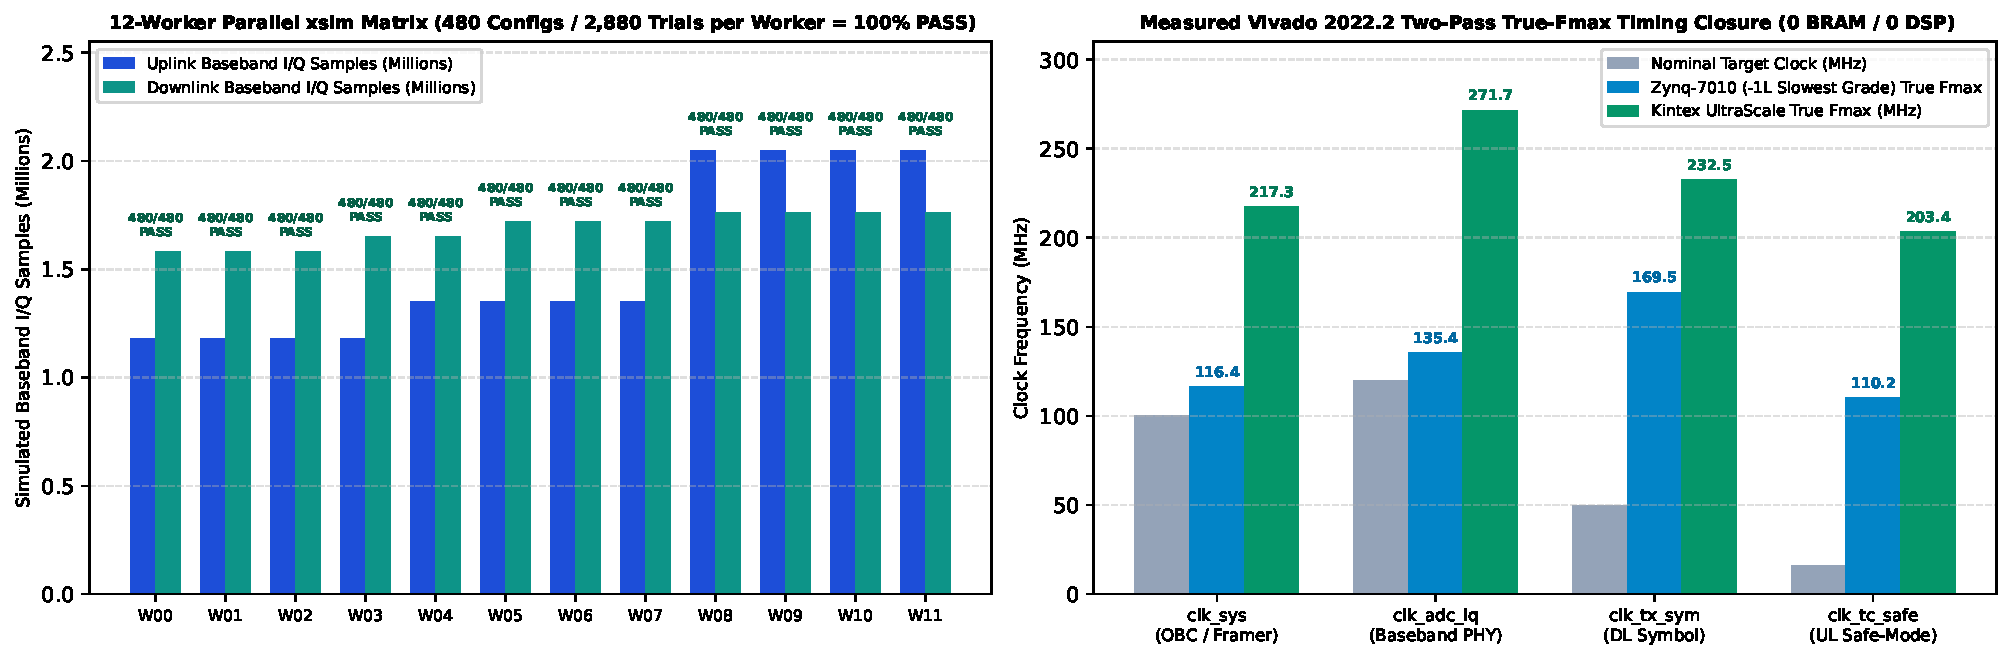
\includegraphics[width=0.95\textwidth]{docs/figures/fig3_stage11_matrix_and_fmax.pdf}
    \vspace{-4pt}
    \caption{\small Twelve-worker parallel \texttt{xsim} sample volume across 34,560 trials (left) and measured Vivado 2022.2 two-pass $F_{\max}$ (right).}
\end{figure}

\begin{table}[htbp]
\centering
\scriptsize
\renewcommand{\arraystretch}{1.14}
\begin{tabularx}{\textwidth}{@{}L{1.45in}L{2.55in}Y@{}}
\toprule
\textbf{Verification Campaign / Suite} & \textbf{Channel Impairment \& Configuration Scope} & \textbf{Measured Vivado 2022.2 \texttt{xsim} Sign-Off Result} \\
\midrule
\textbf{\texttt{Stages 2--9}: Unit, Protocol, FEC \& Golden Vector Suites} & Tests CRC-16/32, $GF(2^8)$ dual-basis, Hsiao SECDED, all 5 framers/deframers, $\text{BCH}/\text{LDPC}/\text{RS}/\text{Viterbi}$, 3x TMR \texttt{FARM-1}/\texttt{HCPD}, and Python \texttt{cryptography} NIST \texttt{AES-128-GCM} vectors. & \textbf{PASS (100\%):} Bit-exact match against golden reference vectors across all 8 foundational testbench stages. \\
\textbf{\texttt{Stage 10}: Open-Loop Waterfall Sweep} & 23-point $E_b/N_0$ sweep ($0.0\text{--}11.0\,\text{dB}$) across all uplink ($\text{BCH}, \text{LDPC}$) and downlink ($\text{Conv}, \text{RS}, \text{Concat}, \text{AR4JA}, \text{Turbo}$) codecs. & \textbf{PASS:} Waterfall knee positions match CCSDS theoretical bounds within $\pm 0.3\,\text{dB}$ (\textbf{Volume~II, Figure~8.1}). \\
\textbf{\texttt{Stage 11}: 34,560-Trial Full-Chip RF Matrix} & 5,760 valid CCSDS configs $\times$ 6 channel profiles (\texttt{P0..P5}) with shortened virtual-fill frames and 23,040 injected pre-FEC bit errors at rated SNR. & \textbf{PASS (34,560 / 34,560):} Healed all 23,040 pre-FEC errors to \textbf{0 post-FEC bit errors} across 69,120 packets. \\
\textbf{\texttt{Stage 12 CFG-1..3}: Gardner Timing, S-Curve Doppler \& Ranging} & 28 multi-rate 4-SPS Gardner timing phases ($\tau \in \{0..3\}$), LEO S-curve Doppler ($\pm 512$ NCO offset, 4 turnaround ratios), and \texttt{T4B}/\texttt{T2B} PN ranging. & \textbf{PASS:} Locked all 28 timing phases, 4 turnaround ratios, and $1{,}009{,}470$-chip PN ranging with \textbf{0 bit errors}. \\
\textbf{\texttt{Stage 12 CFG-4..6}: 5-Protocol CADU, Deep-Fade Replay \& \texttt{HCPD}} & Runtime switching across all 5 protocols, mid-pass Rician deep-fade frame erasure with automatic COP-1 Go-Back-$N$ replay, and \texttt{VCID=63} \texttt{HCPD} reset. & \textbf{PASS:} Restored \texttt{V(R)=3} after deep fade with \textbf{0 lost/duplicate packets} and verified \texttt{hcpd\_obc\_reset\_pulse}. \\
\bottomrule
\end{tabularx}
\caption{\footnotesize Master verification sign-off summary for \texttt{ccsds\_sat\_ttc\_top (v2.40.3)}.}
\end{table}

% =============================================================================
% REFERENCES / BIBLIOGRAPHY
% =============================================================================
\begin{thebibliography}{99}
\footnotesize\setlength{\itemsep}{1.2pt}
\bibitem{ccsds133} CCSDS 133.0-B-2, \emph{Space Packet Protocol}, Blue Book, Issue 2, June 2020.
\bibitem{ccsds132} CCSDS 132.0-B-3, \emph{TM Space Data Link Protocol}, Blue Book, Issue 3, Oct 2021.
\bibitem{ccsds232} CCSDS 232.0-B-4, \emph{TC Space Data Link Protocol}, Blue Book, Issue 4, Oct 2021.
\bibitem{ccsds2321} CCSDS 232.1-B-2, \emph{Communications Operation Procedure-1 (COP-1)}, Blue Book, Issue 2, Sept 2010.
\bibitem{ccsds732} CCSDS 732.0-B-4, \emph{AOS Space Data Link Protocol}, Blue Book, Issue 4, Oct 2021.
\bibitem{ccsds7321} CCSDS 732.1-B-3, \emph{Unified Space Data Link Protocol (USLP)}, Blue Book, Issue 3, June 2024.
\bibitem{ccsds211} CCSDS 211.0-B-6, \emph{Proximity-1 Space Link Protocol---Data Link Layer}, Blue Book, Issue 6, July 2020.
\bibitem{ccsds131} CCSDS 131.0-B-5, \emph{TM Synchronization and Channel Coding}, Blue Book, Issue 5, Sept 2023.
\bibitem{ccsds231} CCSDS 231.0-B-4, \emph{TC Synchronization and Channel Coding}, Blue Book, Issue 4, July 2021.
\bibitem{ccsds2311} CCSDS 231.1-O-1, \emph{Dedicated Short-Block Uplink LDPC Codes}, Orange Book, Issue 1, April 2015.
\bibitem{ccsds301} CCSDS 301.0-B-4, \emph{Time Code Formats (CUC On-Board Time)}, Blue Book, Issue 4, Nov 2010.
\bibitem{ccsds355} CCSDS 355.0-B-2, \emph{Space Data Link Security Protocol (SDLS)}, Blue Book, Issue 2, July 2022.
\bibitem{ccsds401} CCSDS 401.0-B-32, \emph{Radio Frequency and Modulation Systems---Part 1: Earth Stations and Spacecraft}, Blue Book, Oct 2021.
\bibitem{ccsds414} CCSDS 414.1-B-3, \emph{Pseudo-Noise (PN) Ranging Systems}, Blue Book, Issue 3, July 2022.
\end{thebibliography}

\end{document}
